\documentclass{article}
\usepackage[left=1in, right=1in, top=1in, bottom=1in]{geometry}
\usepackage{mathexam}
\usepackage{amsmath}
\usepackage{graphicx,subcaption}
\usepackage{booktabs}
\usepackage{enumitem}
\usepackage{atbegshi}% http://ctan.org/pkg/atbegshi
\usepackage[ruled,linesnumbered]{algorithm2e}
\AtBeginDocument{\AtBeginShipoutNext{\AtBeginShipoutDiscard}}

%\ExamClass{Sample Class}
%\ExamName{Sample Exam}
%\ExamHead{\today}

%\let\ds\displaystyle

\begin{document}

\begin{titlepage}
	\vspace*{\stretch{1.0}}
	\begin{center}
		\Large\textbf{Extended Experiment Report}\\
		\large\textit{05 October 2018}
	\end{center}
	\vspace*{\stretch{2.0}}
\end{titlepage}

%\section{Pruning performance of DiVE-Greedy and DiVE-dSwap}
%
%Note: \textit{Greedy MaxMin and Greedy Top-1 are same, both algorithms have same logic. For the rest of this report, two proposed schemes DiVE-Greedy and DiVE-dSwap will be discussed and both algorithms use Top-1 strategy.} 
%
%\subsection{DiVE-Greedy}
%Similar to the classical Greedy Construction, DiVE-Greedy initializes the set $S$ with the two most distant views.
%%
%Then, DiVE-Greedy iteratively selects new views to be added to $S$. 
%%
%Particularly, in each iteration a view is selected from the set of remaining views in $X$ and is added to $S$.
%%
%The criterion for the view that can be selected is to improve the overal hybrid objective function $F(S)$. 
%%
%Without pruning mechanism, that requires iteration of all candidate views in $X$ to find the best view that can improve $F(S)$ most. While in that process, executing query of each view is needed. 
%%
%To avoid such expensive processing, pruning scheme is proposed. 
%%
%
%\begin{figure}
%	\begin{center}
%		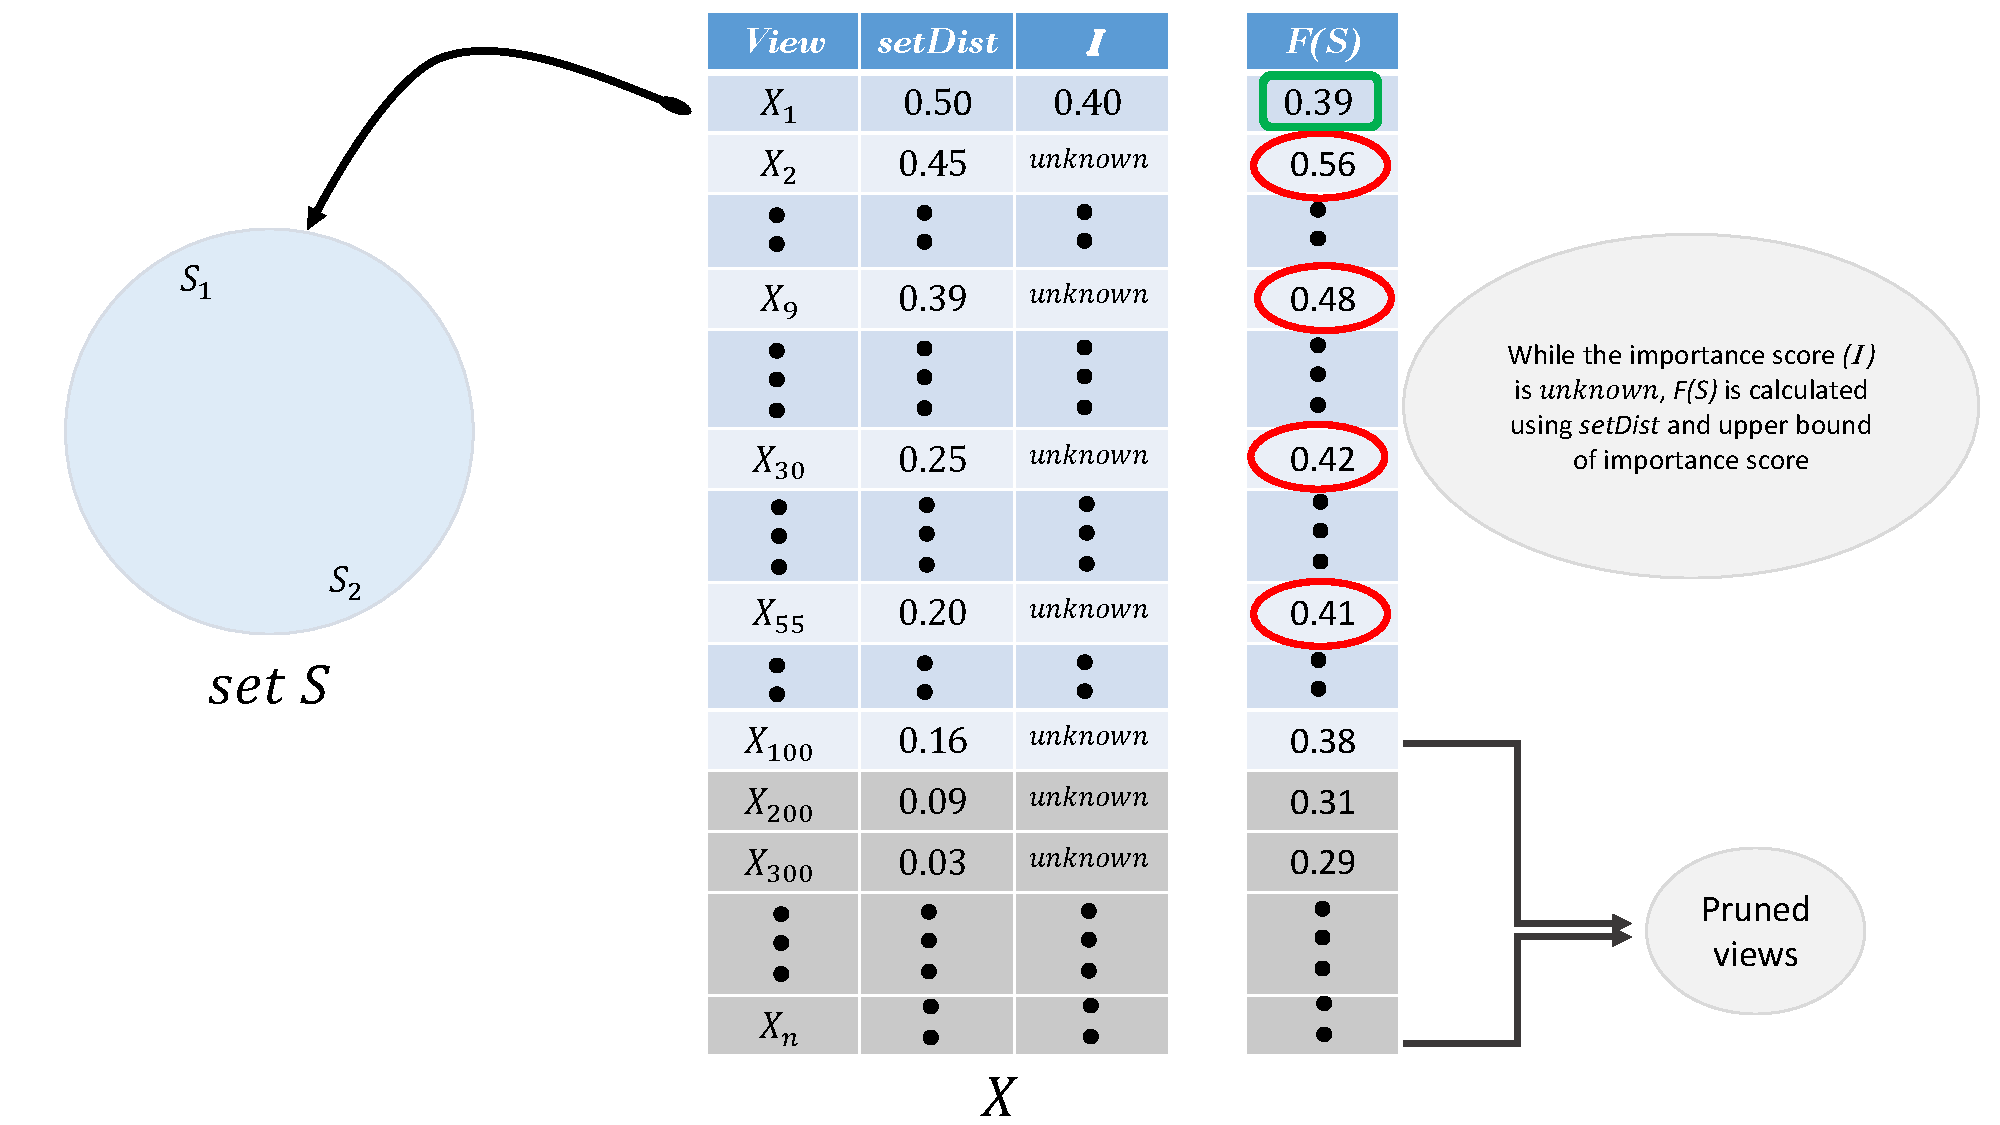
\includegraphics[width=6.0in]{figures/DiVE-Greedy}
%		\vspace{-9pt}
%		\caption{DiVE-Greedy pruning technique}
%		\label{fig:DiVE-Greedy}
%		\vspace{-20pt}
%	\end{center}
%\end{figure}
%
%Our proposed pruning technique is based on the observation that the utility score of each view $U(V_i)$ is a weighted sum of two measures; 1) the importance score of the view (i.e., $I(V_i)$), and 2) the distance of the view from $S$ (i.e., $setDist(V_i, S) $). 
%%
%We note that the computation of $setDist(V_i, S)$ is a CPU-bound (i.e., the execution time is determined by the speed of CPU). 
%%
%To the contrary, computing the importance score of a view $I(V_i)$ is an expensive operation that requires executing two queries (i.e., target and reference data) of $V_i$ (i.e., I/O-bound, where the execution time is determined by the disk speed that more slowly compared to CPU-bound).
%%
%Our pruning technique works by leveraging the diversity score and importance score that allows for pruning low-utility views without incurring the high cost for evaluating their importance as described next.
%%
%\begin{figure}
%	\begin{center}
%		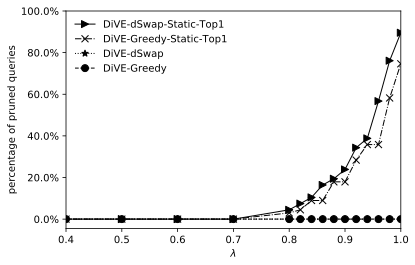
\includegraphics[width=4.0in]{figures/no_pruning_vs_static_extend}
%		\vspace{-12pt}
%		\caption{Static bound pruning performance while different value of $\lambda$, $k = 5$, MaxSum diversification function and running on Fligths dataset}
%		\label{fig:static-pruning}
%		\vspace{-20pt}
%	\end{center}
%\end{figure}
%
%
%For instance, Figure \ref{fig:DiVE-Greedy} shows how DiVE-Greedy pruning works. After the set $S$ are initialized with the two most distant views, $X$ is sorted based on the distance score of candidate views in $X$ to $S$ (i.e., $ setDist(X_i, S) $). The highest score will be on the top (i.e., the highest score of $setDist$ in this example is 0.50). Notice that up to this point there is no query execution, only diversity computation cost (i.e., $ setDist(X_i, S) $) is needed. In order to calculate the $F(S)$, the importance score of view need to be known by executing the query view. To get the importance score of the view, the query view is executed one by one starts from the top. While first view $X_1$ is executed and its importance score has been known (i.e., the importance score of $X_1$ is 0.40), the hybrid objective function can be calculated. The $F(S)$ is the objective function of set $S $ while $X_1$ is added to the set $S$ (i.e., $ F(S \cup X_1) $). This objective function will be the current objective function $ F(S) $ (i.e., 0.39). Then, $ maxF(S \cup X_i) $ of all remaining views in $X$ are calculated using actual diversity score and upper bound of importance score. 
%
%If $ maxF(S \cup X_i) < F(S) $ then it is guaranteed that the actual objective function to be less than the current objective function $ F(S) $ and these views can be pruned (i.e., all views below $X_{100}$ will be pruned). It cannot be denied because the real importance score is always below the upper bound. Meanwhile, if $ maxF(S \cup X_i) > F(S) $ such $X_2 - X_{55}$ (i.e., read circle), these views need to be executed start from the top. If on the next query view execution, there is a view that can improve $ F(S) $ compared to the current $  F(S) $, then the currect $F(S)$ will be updated. This technique is able to prune many low-quality views as shown in Figure \ref{fig:static-pruning}.
%\begin{figure}
%	\begin{center}
%%		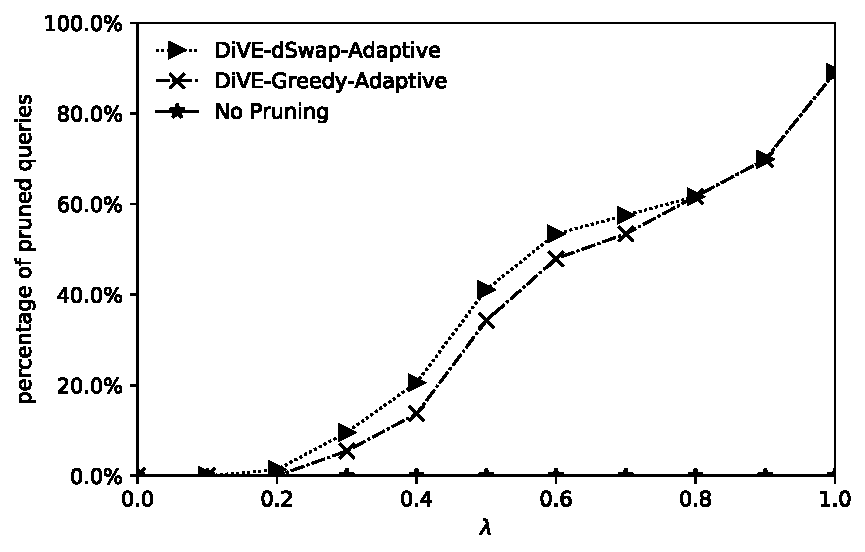
\includegraphics[width=4.0in]{figures/pruning_performance_greedy_dswap_adaptive}
%		\vspace{-12pt}
%		\caption{Adaptive bound pruning performance using different value of $ \lambda $, $k = 5$,  $ PI = 0.97 $, MaxSum diversification, running on Flights dataset}
%		\label{fig:adaptive-pruning-performance}
%		
%	\end{center}
%\end{figure}
%\subsection{DiVE-dSwap}
%As shown in the Figure \ref{fig:static-pruning}, DiVE-Greedy has a good pruning performance even it uses static bound. It will have better performance while adaptive bound is used as shown in Figure \ref{fig:adaptive-pruning-performance}. Although DiVE-Greedy is able to prune many queries, Greedy starts with small number of views (i.e., two most distant views) in the initialization set $S$ that these views cannnot be replaced. Hence, this technique may reducing the quality of recommended views in terms of effectiveness and efficiency. For instance, there is no guarantee that two most distant views which selected by Greedy as the initialization have high importance score and there is no way to replace those two views. Moreover, due to our context-driven only consist of three components (i.e., Attribute, Measure, and Aggregate Function), in the first Greedy iteration many views have same score of $ setDist(X_i, S) $ because only two views are in the set $S$. This issue may decrease the chance of pruning.
%
%In order to overcome these issues, DiVE-dSwap is proposed as well. DiVE-dSwap technique has a replacing mechanism that can replace low quality views in the current set $S$ with the better one. In addition, DiVE-dSwap has bigger number of views in the initialization set $S$ ($|S|$ = $k$). Meanwhile, higher number of views in the set $S$ can decrease the chance of views in $X$ have same $ setDist $ score.  
%
%
%In this experiment, we used Flights dataset with 5 queries, Figure \ref{fig:static-pruning} shows the pruning performance of DiVE-Greedy and DiVE-dSwap while static bound is used and Figure \ref{fig:adaptive-pruning-performance} while adaptive bound is used. 
%


\section{New Dataset}

The student performance dataset is used in this experiment as the motivation example dataset. This dataset can be downloaded from Kaggle \footnote{https://www.kaggle.com/uciml/student-alcohol-consumption} and UCI ML website \footnote{https://archive.ics.uci.edu/ml/datasets/student+performance}. This dataset has 28 attributes, 5 measures, and four aggregate functions are used in this experiments. The data were obtained in a survey of students math and Portuguese language courses in secondary school. It contains a lot of interesting social, gender and study information about students. In this experiment, only math dataset is used. 

For instance, the analyst wants to compare between students who want to continue their study to the higher education and students who do not want to continue their study to higher education. Figure \ref{fig:motivation_dataset} shows two views that have the highest importance score: 1) A = studytime, M = final grade, and F = AVG, the importance score is 0.812831582477977; 2) A = studytime, M = final grade, and F = MAX, the importance score is 0.797221012363291. This Figure shows that without diversity, recommended views may suffer from redundancy. 


Figure \ref{fig:motivation_dataset} also shows that students who want to continue to higher education relatively have better final grade compared to students who do not want to continue to higher education. Interestingly, some students who want to continue their education, they spend more time to study (5 to 10 hours, even more than 10 hours) per week. To contrary, students who do not want to continue their study, all of them only spend less than 5 hours a week for study.


\begin{figure}%
	\centering
	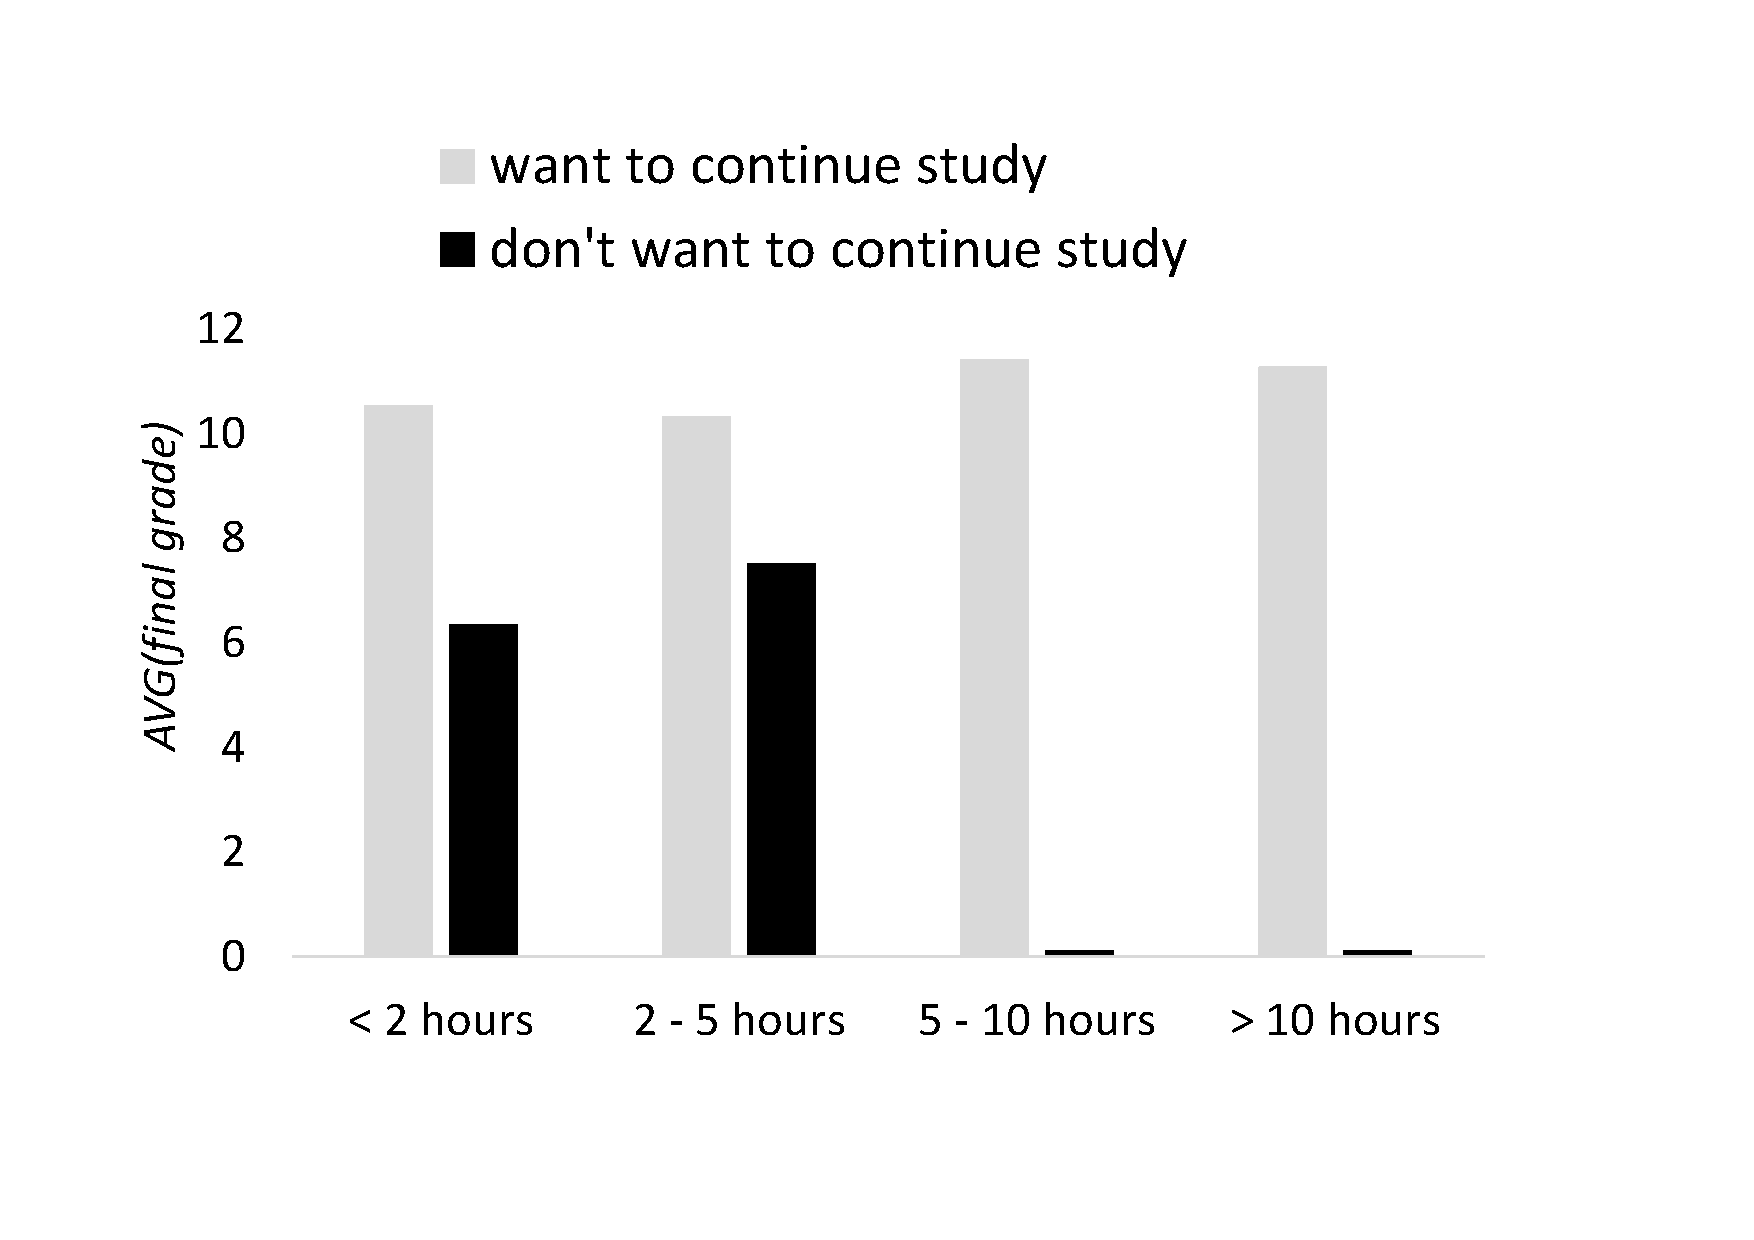
\includegraphics[width=3.2in]{figures/AVG_STUDENT}
	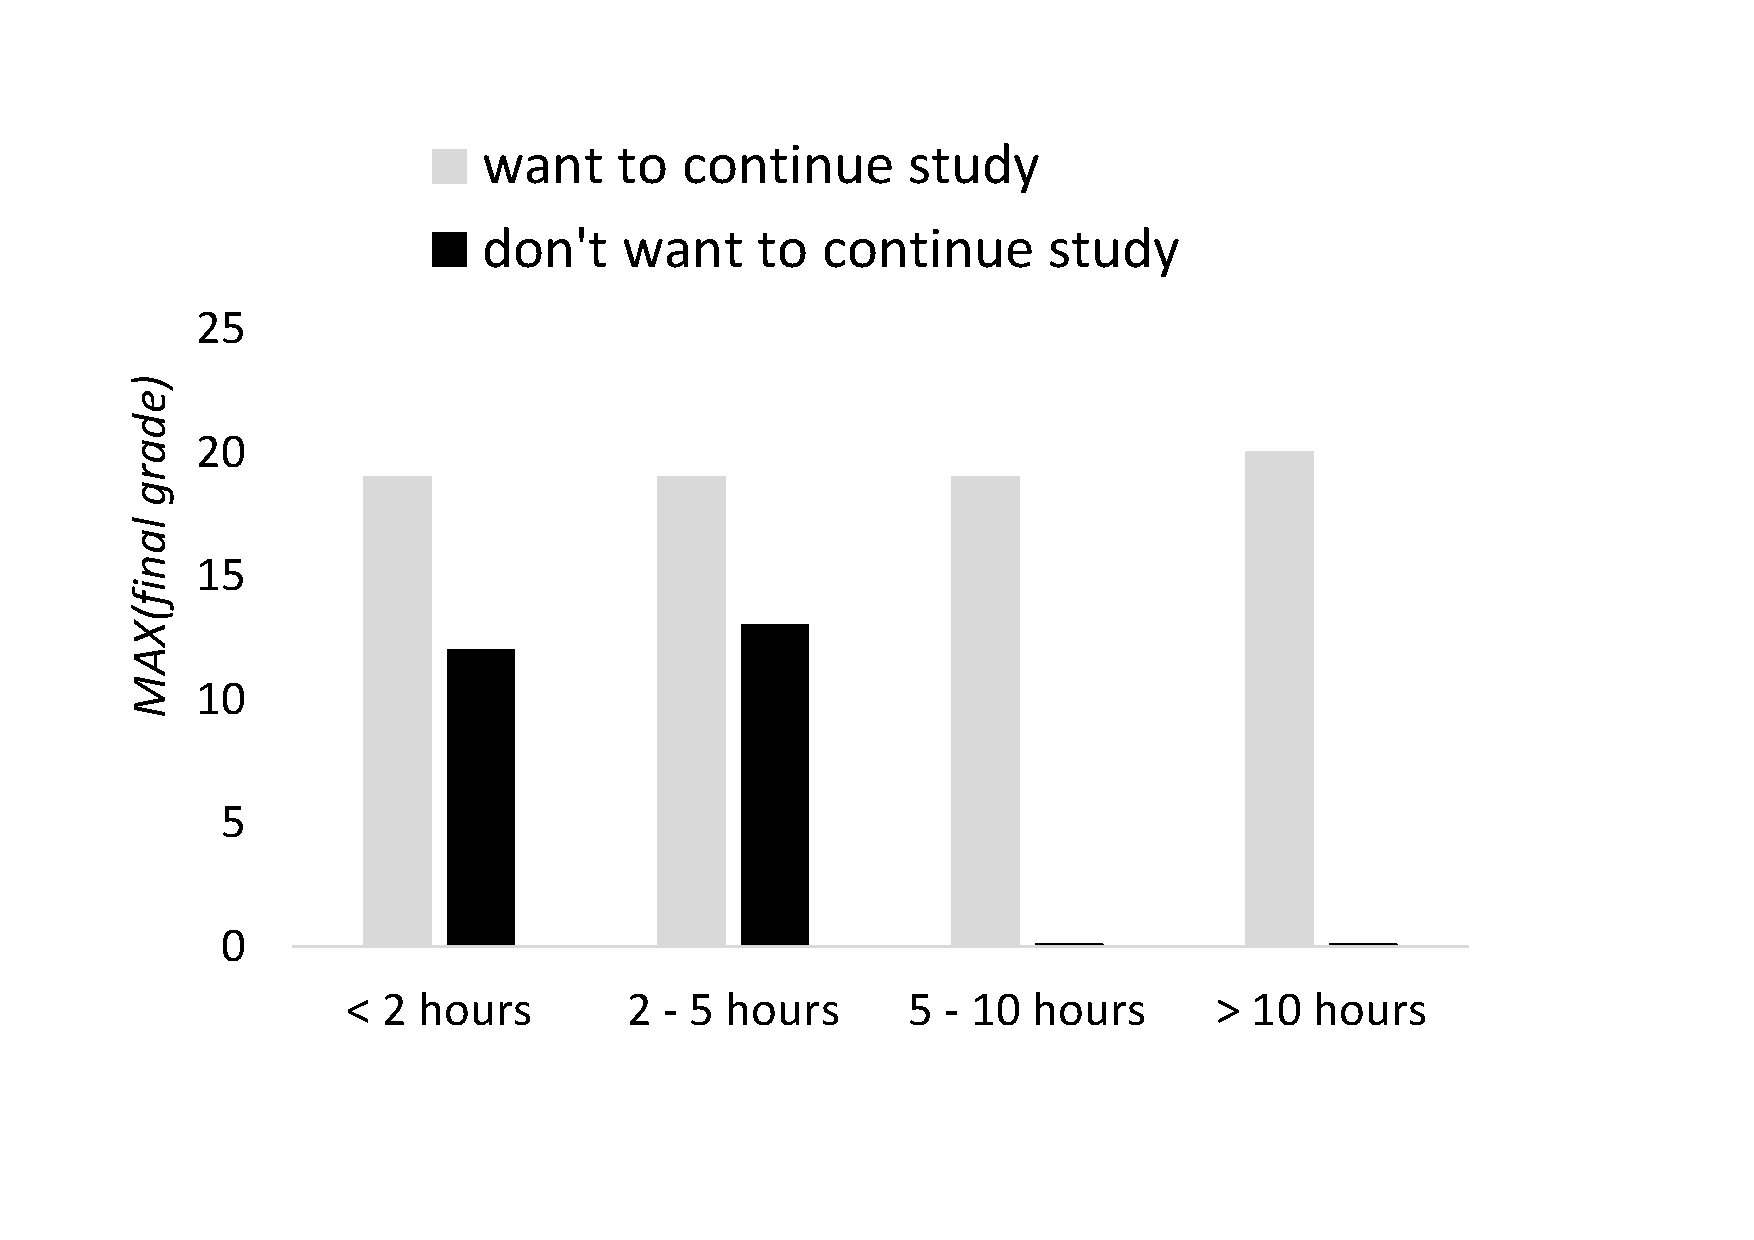
\includegraphics[width=3.2in]{figures/MAX_STUDENT}
	\caption{Study time and final grade of students who want to countinue their study to higher education vs. students who do not want to continue their study to higher education}%
	\label{fig:motivation_dataset}%
\end{figure}

\section{Distance Functions}


There are several distance functions that can be used to compare two probability distributions as follows:

\begin{itemize}
	\item Kullback-Leiber (KL) distance is not bounded, the mathematically proof can be seen below.
	\item Euclidean distance, currently is used and the maximum bound is $ \sqrt{2} $.
	\item Earth Mover Distance (EMD), this distance is widely used and very good for comparing two probability distributions. Mostly this distance used in computer vision application to compare between two histograms. However, this distance is not bounded as well.
	\item Kolmogorov Distance has the maximum bound equal to 1. However, this distance generally is used as hypothesis test that need another parameters such as $\alpha$ and confidence interval. 
\end{itemize}




%a2 + b2 = (a+b)2 - 2ab
%a2-b2 = (a-b)(a+b)
%(a+b)2 = a2+2ab +b2 
%(a-b)2 = a2-2ab +b2 
%(a+b+c)2 = a2 +b2 +c2 +2ab+2bc+2ac



\subsection{Maximum bound of Kullback-Leibler (KL) distance}

For distributions which do not have the same support, KL divergence is not bounded. Look at the definition: $KL(P\vert\vert Q) = \int_{-\infty}^{\infty} p(x)\ln\left(\frac{p(x)}{q(x)}\right) dx$

If $ P $ and $ Q $ have not the same support, there exists some point $x'$ where $p(x') \neq 0$ and $q(x') = 0$, making KL go to infinity. Even both distributions have the same support, when one distribution has a much fatter tail than the other. Then:
$$KL(P\vert\vert Q) = \int p(x)\log\left(\frac{p(x)}{q(x)}\right) \,\text{d}x$$
when
$$p(x)=\overbrace{\frac{1}{\pi}\,\frac{1}{1+x^2}}^\text{Cauchy density}\qquad q(x)=\overbrace{\frac{1}{\sqrt{2\pi}}\,\exp\{-x^2/2\}}^\text{Normal density}$$
then
$$KL(P\vert\vert Q) = \int \frac{1}{\pi}\,\frac{1}{1+x^2} \log p(x) \,\text{d}x + \int \frac{1}{\pi}\,\frac{1}{1+x^2} [\log(2\pi)/2+x^2/2]\,\text{d}x$$
and
$$\int \frac{1}{\pi}\,\frac{1}{1+x^2} x^2/2\,\text{d}x=+\infty$$


\subsection{Euclidean Maximum bound}
For the general case, Euclidean distance $d$ is defined as following: 
$d = \sqrt{\sum{(x-y)^2}}$, where $ \sum{(x-y)^2} = \sum x^2 + \sum y^2 - 2\sum xy$. Given that in probability vectors all values are nonnegative, $d$ is max when the last term is zero, then $d = \sum x^2 + \sum y^2$. All values are between 0 and 1 (sum up to 1), $\sum x = \sum y = 1$. The theoretical maximum is attained when $2\sum xy = 0$ and $\sqrt{2}$ as the maximum theoretical bound can be proven as following: 
\newline
$ \sqrt{\sum{(x-y)^2}} \leq \sqrt{\sum{(x)^2} + \sum{(y)^2}} $
\newline
$ \sqrt{\sum{(x-y)^2}} \leq \sqrt{1 + 1} $
\newline
$ \sqrt{\sum{(x-y)^2}} \leq \sqrt{2} $


\section{Max-sum and Max-min diversification}
The main objective of diversity is to select a set $ S $  from a given set $ \mathbf{V} $ in such a way that the diversity among the selected elements in set $ S $ is maximized. All experiments that have been done are using MaxSum diversification as the diversity function. Whereas, there is another function of diversification which is MaxMin diversification. In this section, both diversification functions will be discussed, 

MaxSum uses average score of diversity of the set $ S $ which is by computing the total sum of all distances then dividing by $ k*(k-1) $ while the objective of MaxMin is to maximize of minimum score of distance among all points in the set $ S $.  Hence, the range diversity score from those both approaches are different. For instance, there are three views in set $ Z $ which each view is different with others. The maximum score of distance between two views is $ 1 $ and the minimum is $ 0 $. Using MaxSum method the diversity score of set $ Z $ will be $ (1+1+1)/(3*(3-1)) = 0.5 $ whereas diversity score of MaxMin is $ 1 $ because the minimum distance in the set $ Z $ is $ 1 $. 


\begin{figure}
	\begin{center}
		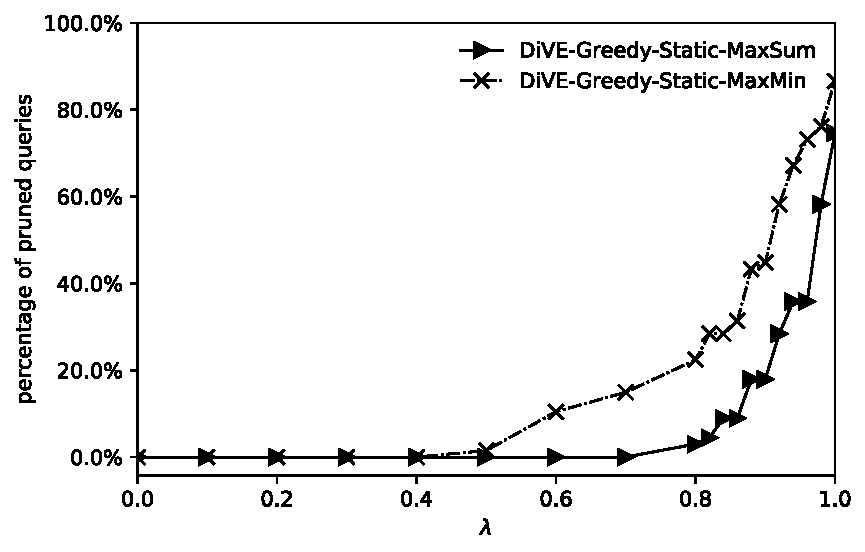
\includegraphics[width=3.0in]{figures/MaxSum_MaxMin_Greedy}
		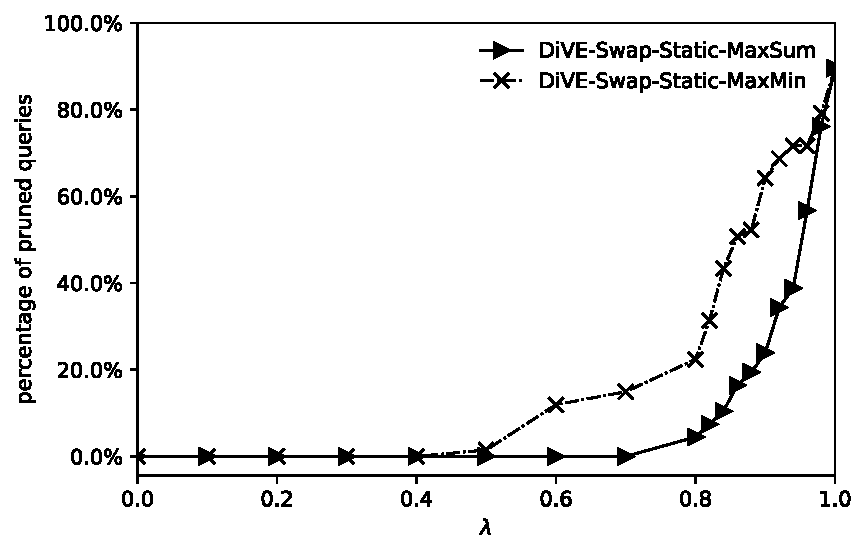
\includegraphics[width=3.0in]{figures/MaxSum_MaxMin_Swap}
		\caption{MaxSum vs. MaxMin diversification on Greedy and Swap running on Flights dataset, $k = 5$}
		\label{fig:maxsum-maxmin-greedy-swap}
	\end{center}
\end{figure}




The example variance of $ setDist $ score using Flights dataset between MaxSum diversification and MaxMin diversification can be seen in the Table \ref{tab:setDist-score}. In this experiment, I selected two most distant views as the initial set $ S $ and then calculate the $ setDist $ of all views in $ X $. For instance, the highest score of $ setDist $ is $ v1 $, where on MaxSum the maximum sore is $ 0.5 $ and on MaxMin the maximum score is $ 1 $. This Table is just an example, in the real data there are many views have same score. In this Table, I only want to show the distributions of $ setDist $ score and the different range of $ setDist $ score between MaxSum and MaxMin. 

\begin{table}
	\begin{center}
		\caption{Example setDist score}
		\label{tab:setDist-score}
		\begin{tabular}{ccl}
			\toprule
			$ v $ in $ X $ &MaxSum &MaxMin\\
			\midrule
			$ v_1 $ & 0.5 & 1.0\\
			$ v_2 $ & 0.472222222 & 0.833333333\\
			$ v_3 $ & 0.444444444 & 0.666666667\\
			$ v_4 $ & 0.4166666667 & 0.5\\
			$ v_5 $ & 0.3899999999 & 0.333333333\\
			$ v_6 $ & 0.3611111111 & 0.166666667\\
			$ v_7 $ & 0.3333333333 & 0.166666667\\
			\bottomrule
		\end{tabular}
	\end{center}
\end{table}


Due to this different diversity score, MaxMin diversification can improve the pruning performance as shown in the Figure \ref{fig:maxsum-maxmin-greedy-swap}. However, this MaxMin makes unbalance between the importance score and diversity score. The maximum diversity can be equal to $ 1 $ while the value of importance score is lower than that. This thing makes the shape of objective function unbalance as shown in Figure \ref{fig:Objective-function-maxsum-maxmin}.
\begin{figure}
	\begin{center}
		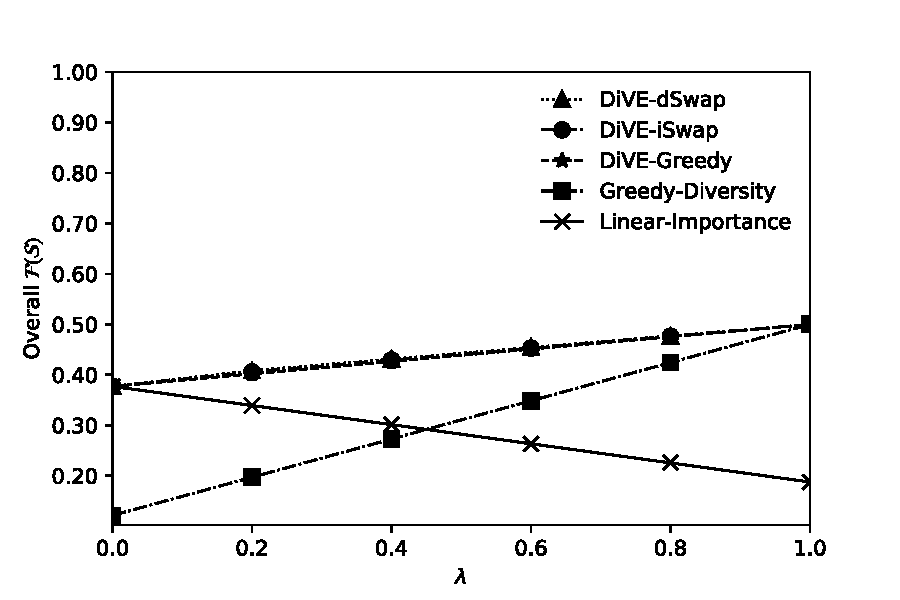
\includegraphics[width=3.0in]{figures/1_tradeoff_June_objf_disease_maxSUM}
		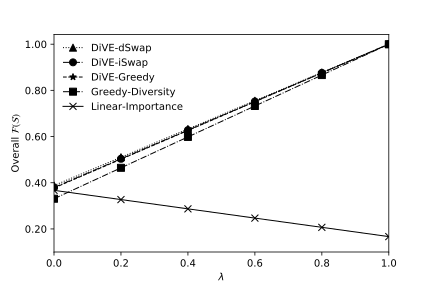
\includegraphics[width=3.0in]{figures/1_tradeoff_June_objf_disease_MaxMIN}
		\caption{Objective function shape on MaxSum vs. MaxMin diversification while different value of $\lambda$, $k = 5$}
		\label{fig:Objective-function-maxsum-maxmin}
	\end{center}
\end{figure}




\section{Impact of $ k $ to pruning performance}


To observe the impact of $k$ to pruning performance while the $\lambda$ is constant, we run DiVE-Greedy-Adaptive and DiVE-dSwap-Adaptive on Flights dataset, using 5 queries, $\lambda = 0.5$ and different value of $k$. Figure \ref{fig:impact-of-k-pruning-performance} shows the result of both schemes. Overall, the pruning performance is decreasing while $k$ is increasing. This result follows the expectation, while $k$ increase, the number of iteration will be increased. Increasing the number of iterations means more views need to be executed and less views are pruned. 
\begin{figure}
	\begin{center}
		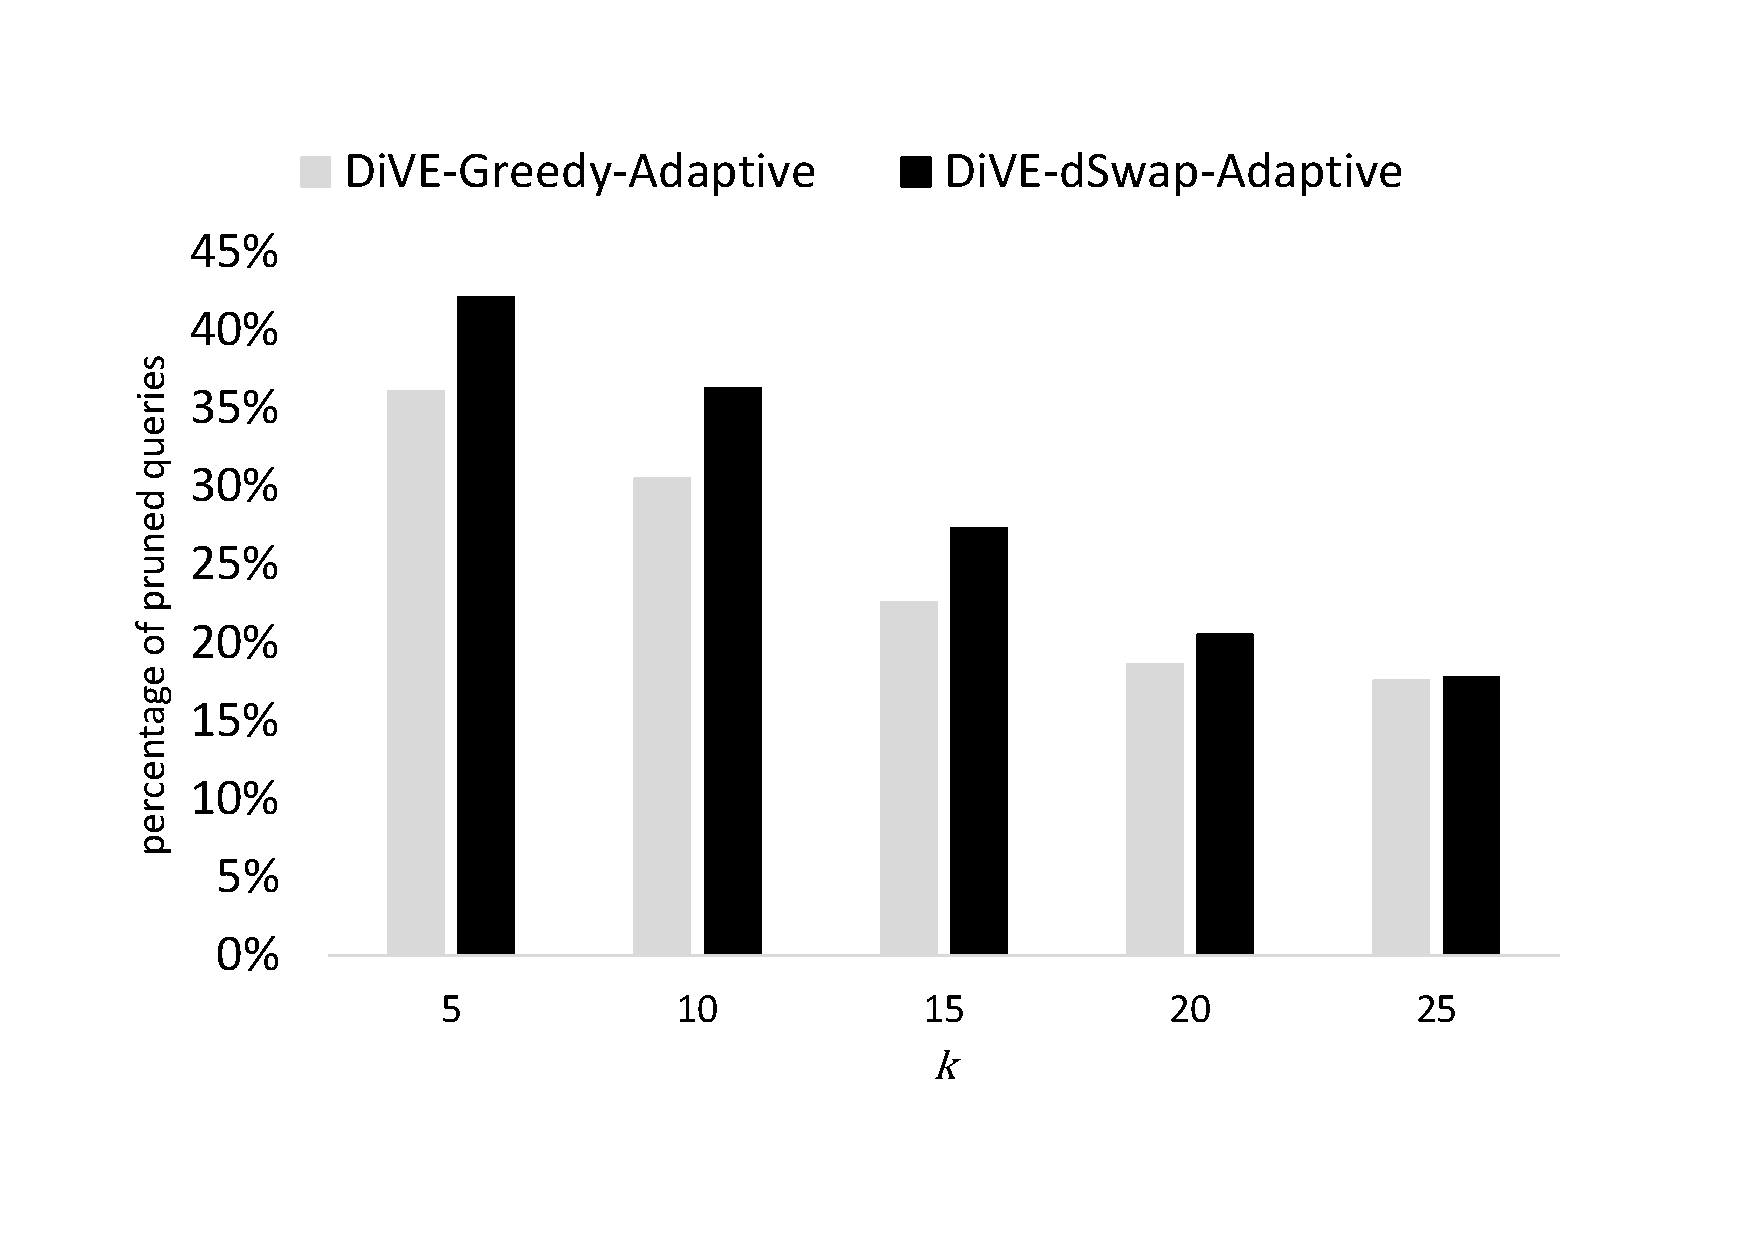
\includegraphics[width=4.0in]{figures/Impact_k_performance}
		\vspace{-30pt}
		\caption{Impact of $k$ to pruning performance, $\lambda = 0.5$, MaxSum diversification, running on Flights dataset}
		\label{fig:impact-of-k-pruning-performance}
		
	\end{center}
\end{figure}

Moreover, There are some interesting finding from Figure \ref{fig:impact-of-k-pruning-performance}. Overall, DiVE-dSwap-Adaptive has better performance compared to DiVE-Greedy-Adaptive in terms of the number of pruned queries. This is because the diversity of $setDist$ score. In case of DiVE-Greedy-Adaptive, no matter how many views inside the set $S$ (i.e., size of $k$), Greedy always start with two most distant views as the initialization set $S$. Consequently, there will be many candidate views in $X$ have same $setDist$ score in the first Greedy iteration that may reduce the chance of pruning (i.e., the effect of diversity of $setDist$ score). Meanwhile,  DiVE-dSwap-Adaptive has higher number of views in the initialization set $S$ (i.e., in this experiment, we used $k = 5$ as the minimum). Hence, the $setDist$ score on DiVE-dSwap-Adaptive is more diverse than DiVE-Greedy-Adaptive in the first iteration and next iteration as well. 

To confirm that, we did experiments that the results can be seen in the Figure \ref{fig:impact-of-k-pruning-performance}. Figure \ref{fig:impact-of-k-pruning-performance} shows DiVE-dSwap-Adaptive has better performance compared to DiVE-Greedy-Adaptive. However, DiVE-Greedy-Adaptive and DiVE-dSwap-Adaptive have almost same number of pruned queries while the number of $k$ is small such as $k=3$. While $k=3$, Greedy has two most distant views in the initialization set $S$ and it only needs one Greedy iteration to generate the recommended views. Meanwhile, Swap has three views as the initialization, it needs to exchange the candidate views in $X$ to set $S$ until the set $S$ has the optimal $F(S)$. In this case, both algorithms will have same condition in terms of $setDist$ calculation (i.e., the distance between each view in $X$ to two views in set $S$). Hence, the Figure shows both algorithms have same performance while $k = 3$. This results indicate that the diversity of $setDist$ scores affects the performance of pruning. 



%In this condition, the diversity of $setDist$ score of both algorithms are same.  
%
%Almost in all $k$, DiVE-dSwap-Adaptive has better performance compared to DiVE-Greedy-Adaptive in terms of the number of pruned queries. This is because of the number of initialization set $S$, as shown in the Figure while the number of initialization set is close such as $k = 3$, both algorithms have close performance and the gap is higher while $k$ is increasing. The number of initialization set $S$ causes the diversity of $setDist$ score. 
%
%
%Moreover, both algorithms also have close number of pruned queries while the number of $k$ is high such as $k=25$. 







\section{Total cost with and without pruning}
To see the performance of our proposed pruning approach, especially compared to schemes without pruning, Figure \ref{fig:flight_costs_all} shows the total cost running on Flights dataset. As shown in the Figure, DiVE-Greedy-Adaptive and DiVE-dSwap-Adaptive are able to reduce query cost. This experiment using adaptive algorithm while $ PI = 0.97 $ and this result is the avarage from five queries on Flights dataset. 


\begin{figure}
	\begin{center}
		\vspace{-50pt}
		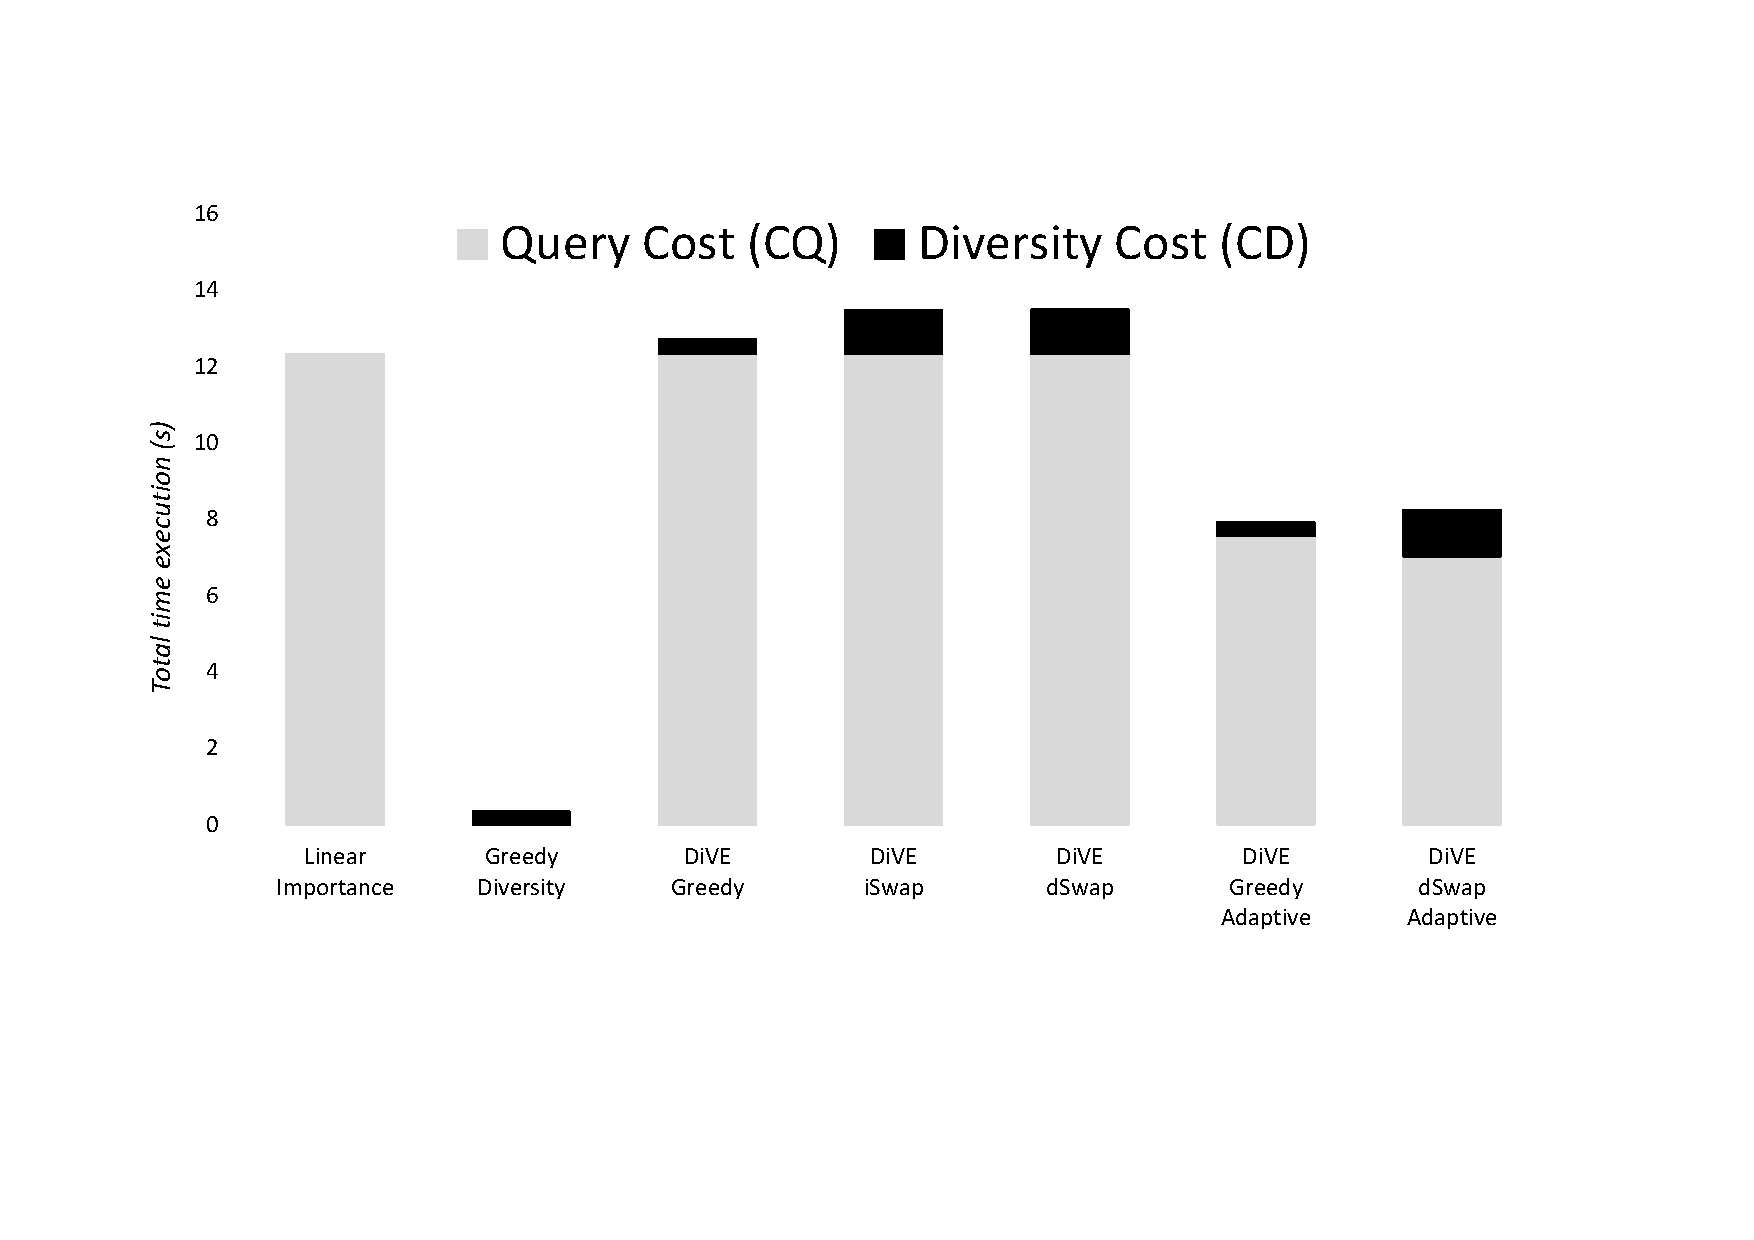
\includegraphics[width=7.0in]{figures/flight_costs_all}
		\vspace{-90pt}
		\caption{Total costs of schemes running on Flights dataset, MaxSum diversification, $k = 5$,  $ PI = 0.97 $, and $\lambda = 0.5$ }
		\label{fig:flight_costs_all}
		\vspace{-20pt}
	\end{center}
\end{figure}

\section{DiVE-Greedy and DiVE-Swap complexity}
The costs of Greedy Construction algorithm has two components which are the query execution cost $C_Q$ that computing the importance score of view and the diversity cost $C_D$ that computing set distance of each view from the views already in S. The complexity of query execution cost is $ O$($n$) as the content of each view is generated only once. The diversity cost $C_D$ is $ O$($kn$) where $k$ is the size of subset of views $ S $ and $ n $ is the number of all possible views.


Meanwhile, The costs of Swap algorithm is also depend on the query execution time $C_Q$ of all possible views and the diversity computation $C_D$. The query cost $C_Q$ is executed only once but the cost is high due to it needs I/O cost. However, the complexity of diversity computation $C_D$ is $ O\left(k^2n \right) $ and the number of distance computation depends on the number of iterations of the swap and the number of views in $X$. In the worst case, swap algorithm can perform $ O\left(k^n \right) $. 

%The different of total cost between Greedy and Swap approach can be seen in Figure \ref{fig:flight_costs_all}. Meanwhile, the impact of $k$ to the distance computation time while running on Flights dataset can bee seen in Figure \ref{fig:impact-of-k-diversity-computation}.


\begin{algorithm}
	\SetAlgoVlined
	\DontPrintSemicolon
	%This is to hide Begin keyword
	\SetKwBlock{Begin}{}{end}
	\KwIn{Set of views V and result set $S$ize k }
	\KwOut{Result set $ S \geq V $, size S = k}  
	\SetKwFunction{FgetL}{getL}
	$S \leftarrow $ two most distant views\;
	$X \leftarrow  \left[V \backslash S\right]$\;
	
	
	
	\SetKwFunction{FgetL}{getL}
	\SetKwProg{Fn}{function}{:}{}
	\Fn{\FgetL{$f$,$S$, $X$,$L$}}{
		\For{$X_i$ in set $X$}{
			\For{$S_j$ in set $S$}{
				$ d  \leftarrow setDist\left(X_i,S \right) $\;
				$ 	X' \leftarrow [ X_i, d]$\;
				$ 	L.append(X')$\;
			}
		}
		$ 	L \leftarrow sorted\_by\_d(L) $\;
		
		\KwRet\;
	}
	
	$maxI, max_b \leftarrow 0, \sqrt{2} $\;
	$ rectify \leftarrow False $\;
	$ S_{rectify}, L_{rectify}   \leftarrow S, getL(S,X) $\;
	\;
	\While{$i < k$}{
		\If{$ max_b == \sqrt{2}$}{
			$samples \leftarrow get\_samples(PI)$\;
			$maxI\_S \leftarrow get\_maxI(S)$\;
			$maxI\_samples \leftarrow get\_maxI(samples)$\;
			
			\If{ $ maxI\_S > maxI $}{
				$ maxI \leftarrow maxI\_S$
			}
			\If{ $ maxI\_samples> maxI $}{
				$ maxI \leftarrow maxI\_samples$
			}
			$max_b \leftarrow maxI$			
			
		}
		
		$ S' \leftarrow S $\;
		$ L \leftarrow getL(S,X) $\;
		
		
		
		\For{$L_i$ in $L$}{
			
			\If{ $ F\left(S'\right) < F\left(S \cup X_i, max_b\right) $}{
				$ 	L'.append(L_i)$\;
			}
			$ I \leftarrow get\_I\_score(L'_i) $\;
			\If{ $ F\left(S'\right) < F\left(S \cup X_i, I\right) $}{
				$ S'  \leftarrow S \cup X_i $  \;
			}
			\eIf{ $ I > max_b $}{
				$ max_b \leftarrow I $\;
				$ rectify = True $\;
				$ break (Out\ of\ Loop) $\;
			}{
				$ rectify = False $\;
			}
			
		}
		
		
		
		\eIf{rectify == True}{
			$ S, S' \leftarrow S_{rectify} $ \;
			$ L \leftarrow L_{rectify} $ \;
			$i \leftarrow  len(S)$ \;
			
			
		}{
			
			
			\If{ $ F\left(S'\right) > F\left(S\right) $}{
				$ S  \leftarrow S'$\;
				
			}
			$i = i + 1  $
			
		}
	
		
		%
		%\If{ $ F\left(S'\right) > F\left(S\right) $}{
		%	$ S  \leftarrow S'$
		%	$  improve \leftarrow  True $\;
		%	
		%	}{
		%		$improve \leftarrow  False $\;
		%	
		%	}
	}
	$return S$
	\caption{\textit{DiVE} Greedy Pruning Rectifying}\label{DiVE-Greedy-Pruning-Rectifying}
\end{algorithm}


% Pruning Pseudocode

\begin{algorithm}
	\SetAlgoVlined
	\DontPrintSemicolon
	%This is to hide Begin keyword
	\SetKwBlock{Begin}{}{end}
	\KwIn{Set of views V and result set $S$ize k }
	\KwOut{Result set $ S \geq V $, size S = k}  
 	\SetKwFunction{FgetL}{getL}
	$S \leftarrow $ Result set of only diversity\;
	$X \leftarrow  \left[V \backslash S\right]$\;

	
	
	\SetKwFunction{FgetL}{getL}
	\SetKwProg{Fn}{function}{:}{}
	\Fn{\FgetL{$f$,$S$, $X$,$L$}}{
		\For{$X_i$ in set $X$}{
			\For{$S_j$ in set $S$}{
				$ d  \leftarrow setDist\left(X_i,S \backslash S_j\right) $\;
				$ 	X' \leftarrow [S_j, X_i, d]$\;
				$ 	L.append(X')$\;
			}
		}
		$ 	L \leftarrow sorted\_by\_d(L) $\;
		
		\KwRet\;
	}

$F_{current}, maxI, max_b \leftarrow 0, 0, \sqrt{2} $\;
$  improve, rectify \leftarrow  True, False $\;
$ S_{rectify}, L_{rectify}   \leftarrow S, getL(S,X) $\;
	\;
	\While{improve = True}{
		\If{$ max_b == \sqrt{2}$}{
			$samples \leftarrow get\_samples(PI)$\;
			$maxI\_S \leftarrow get\_maxI(S)$\;
			$maxI\_samples \leftarrow get\_maxI(samples)$\;
			
			\If{ $ maxI\_S > maxI $}{
				$ maxI \leftarrow maxI\_S$
			}
			\If{ $ maxI\_samples> maxI $}{
				$ maxI \leftarrow maxI\_samples$
			}
			$max_b \leftarrow maxI$			
			
		}
	
		$ S' \leftarrow S $\;
		$ L \leftarrow getL(S,X) $\;
		
		
		
		\For{$L_i$ in $L$}{
			
			\If{ $ F\left(S'\right) < F\left(S \backslash S_j \cup X_i, max_b\right) $}{
				$ 	L'.append(L_i)$\;
			}
			$ I \leftarrow get\_I\_score(L'_i) $\;
			\If{ $ F\left(S'\right) < F\left(S\backslash S_j \cup X_i, I\right) $}{
				$ S'  \leftarrow S \backslash j \cup X_i $  \;
			}
			\eIf{ $ I > max_b $}{
				$ max_b \leftarrow I $\;
				$ rectify = True $\;
				$ break (Out\ of\ Loop) $\;
			}{
			$ rectify = False $\;
		}
			
		}
		
		
		
		\eIf{rectify == True}{
			$ S, S' \leftarrow S_{rectify} $ \;
			$ L \leftarrow L_{rectify} $ \;
			$improve \leftarrow  True$ \;
			
			
		}{
			
			
			\If{ $ F\left(S'\right) > F\left(S\right) $}{
				$ S  \leftarrow S'$\;
				
			}
			
			\eIf{ $ F\left(S\right) > F_{current} $}{
				$ F_{current}  \leftarrow F\left(S\right) $\;
				$  improve \leftarrow  True $\;
				
			}{
				$improve \leftarrow  False $\;
				
			}
			
		}
		
		%
		%\If{ $ F\left(S'\right) > F\left(S\right) $}{
		%	$ S  \leftarrow S'$
		%	$  improve \leftarrow  True $\;
		%	
		%	}{
		%		$improve \leftarrow  False $\;
		%	
		%	}
	}
	$return S$
	\caption{\textit{DiVE} dSwap Pruning Rectifying}\label{DiVE-dSwap-Pruning-Rectifying}
\end{algorithm}




\section{Correcting wrong maximum bound in adaptive pruning scheme}


As explained in the first section, DiVE schemes utilize the importance score bound to do pruning. There are two techniques proposed: 1) static bound and 2) adaptive bound. In the static bound, the theoritical maximum bound ($ \sqrt{2} $) is used and this bound will not be changed until the end of running. Meanwhile, adaptive used the theoritical maximum bound ($ \sqrt{2} $) as the first, then this bound is updated while the maximum bound of actual importace score of views has been known. 


In order to know when the bound should be updated, samping based on prediction interval is used. Before running the program, user needs to defined what PI that she wants to use. For instance, while users set PI to 80 means after 9 views are executed, then the current bound will be updated to the maximum importance score which have seen so far. Generally, PI can be defined as following: 

\begin{itemize}[noitemsep]
	\item PI80: need to execute 9 views
	\item PI85: need to execute 12 views
	\item PI90: need to executes 20 views
	\item PI95: need to executes 40 views
	\item PI97: need to executes 60 views
\end{itemize}

%
%\begin{figure}
%	\begin{center}
%		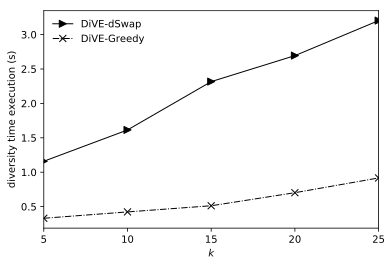
\includegraphics[width=4.0in]{figures/impact_of_k_to_diversity_cost}
%		\vspace{-12pt}
%		\caption{Impact of $k$ to diversity computation running on Flights dataset}
%		\label{fig:impact-of-k-diversity-computation}
%		
%	\end{center}
%\end{figure}
%
%
%
%\begin{figure}
%	\begin{center}
%		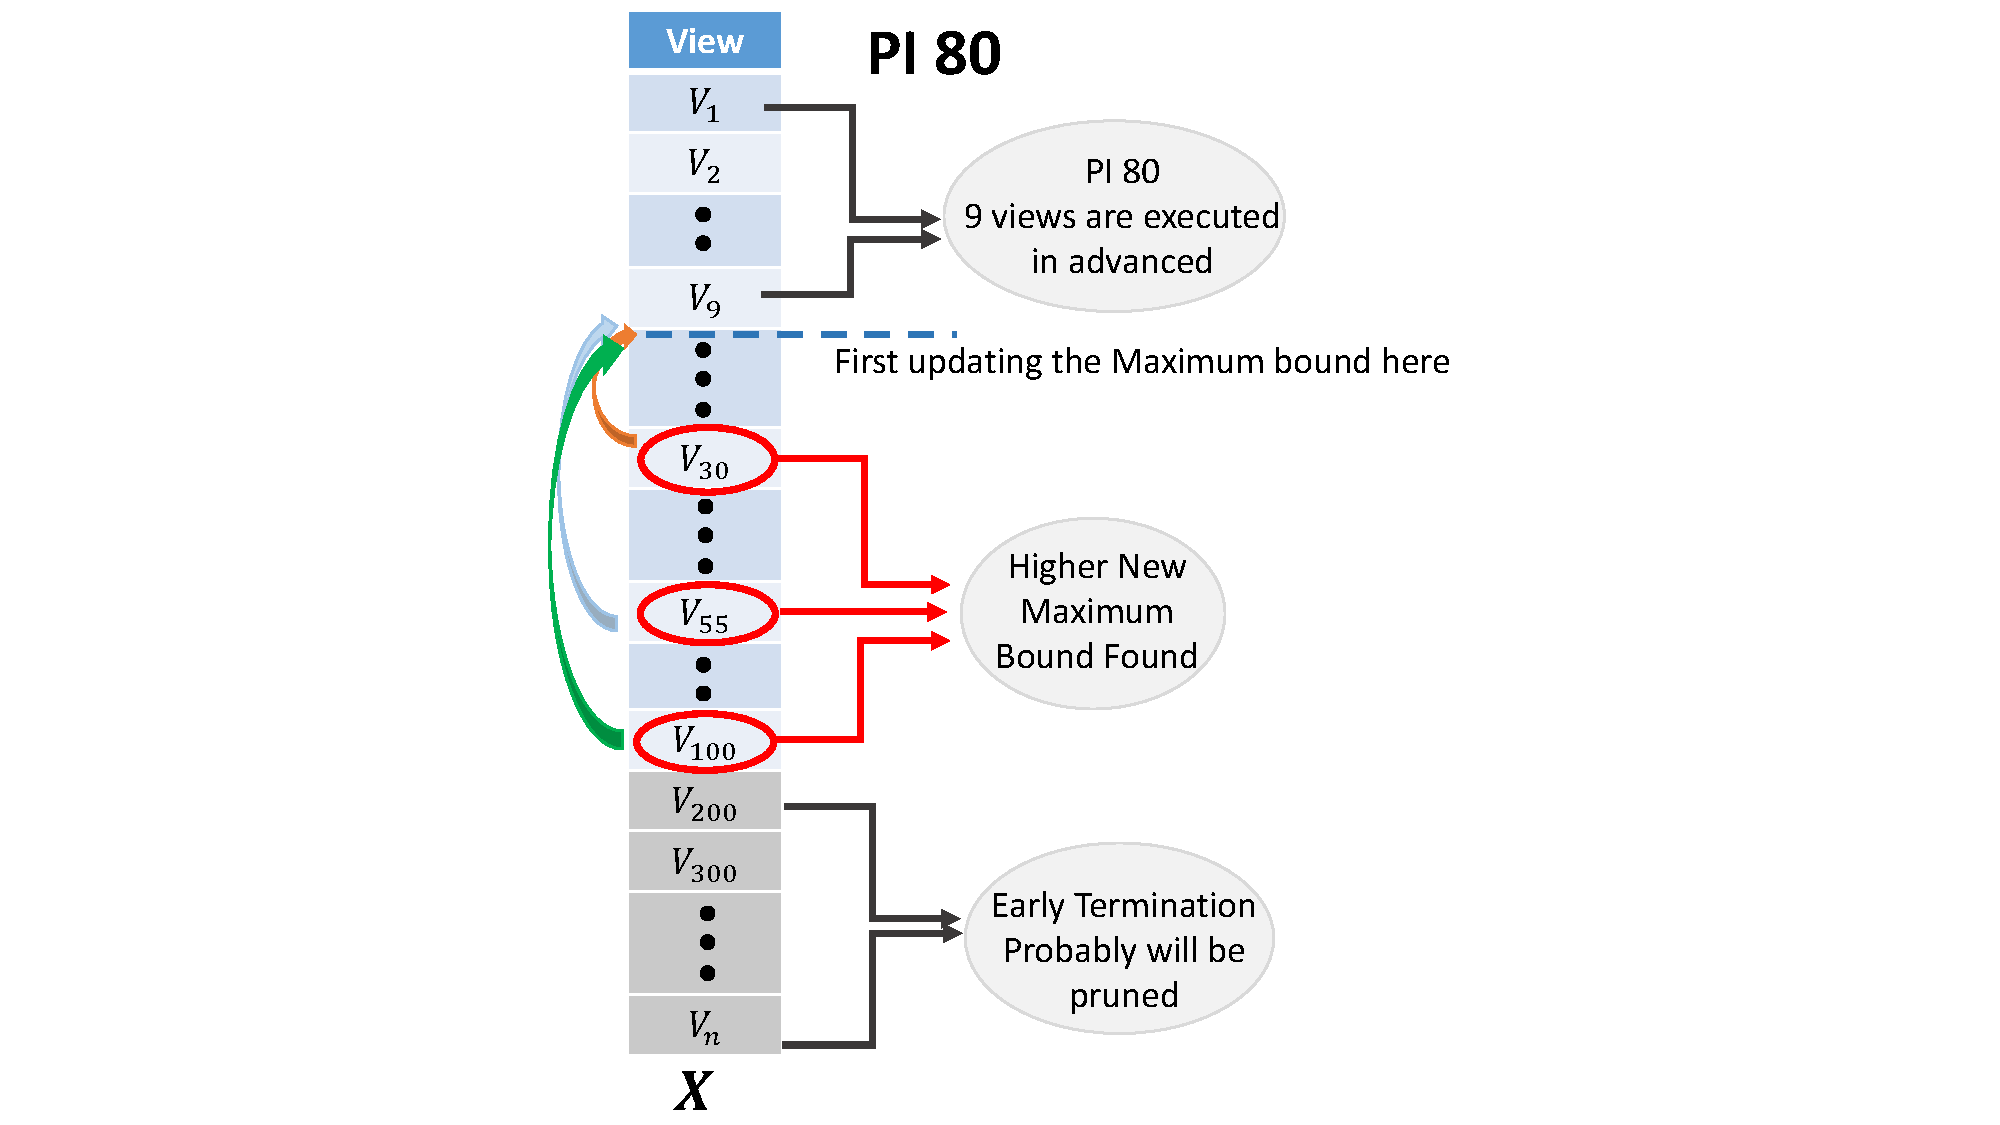
\includegraphics[width=7.0in]{figures/rectifying_bound_2}
%		\vspace{-8pt}
%		\caption{Rectifying maximum bound on adaptive pruning scheme}
%		\label{fig:rectifying_bound_2}
%		
%	\end{center}
%\end{figure}


%As shown in the Figure \ref{fig:DiVE-Greedy} and \ref{fig:adaptive-pruning-performance}, the adaptive bound has a better performance of pruning compared to the static one. 

Adaptive scheme has the best pruning performance while PI80 is used. However, it reduces the effectiveness of recommended views due to only small number of executed views are needed for PI80 which increase probability to have wrong bound. It can be shown in Figure \ref{fig:pruning_performance_swapd}, the error $F(S)$ on Adaptive Pruning. As shown in the Figure, the safest way is to use higher PI such as PI97. However, if there is a way to keep using PI80 without reducing effectiveness, it will definitely be very good. In fact, the goal of pruning scheme is to minimize query view execution (i.e., use low PI) without reducing the quality of recommended views. 
\begin{figure}
	\begin{center}
		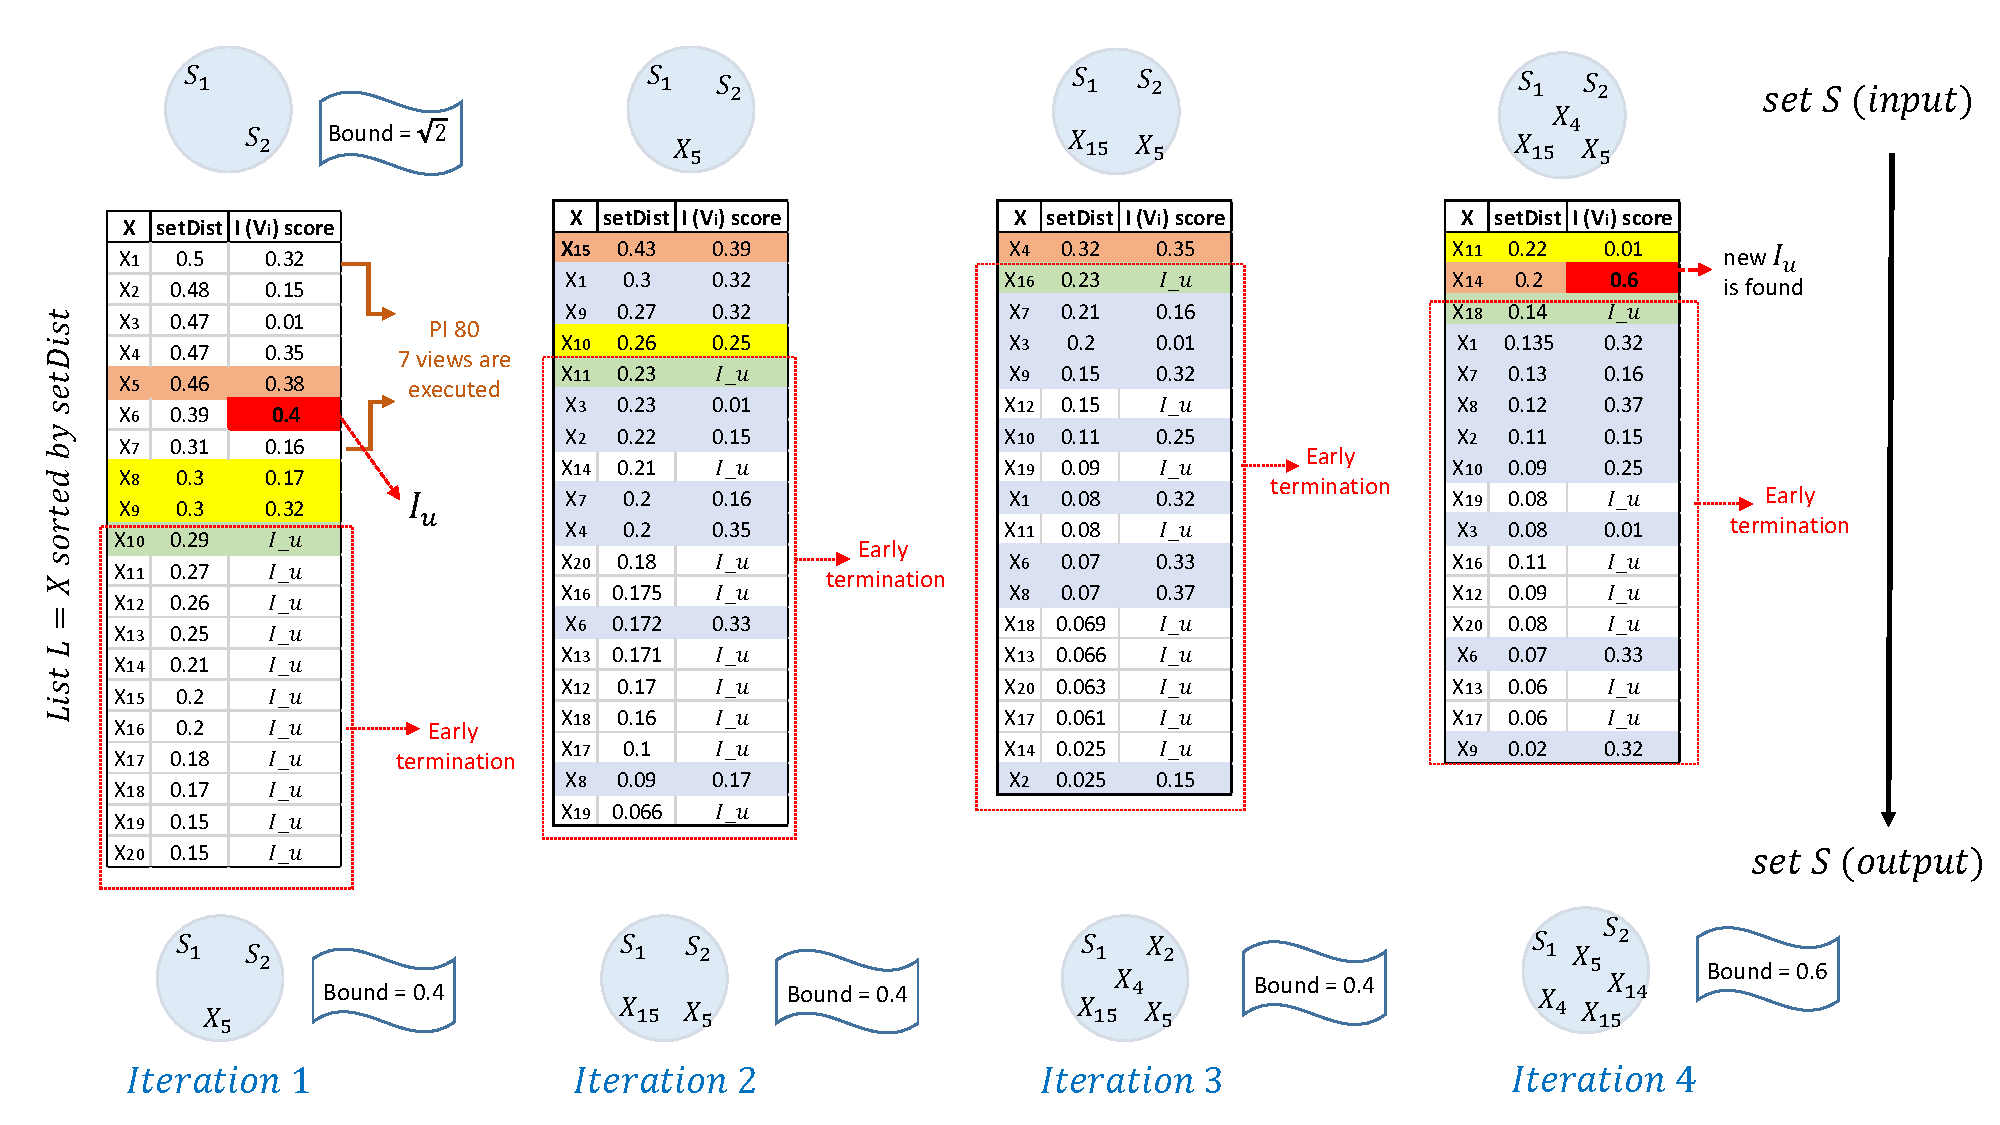
\includegraphics[width=5.0in]{figures/Rectifying_flow_column}
%		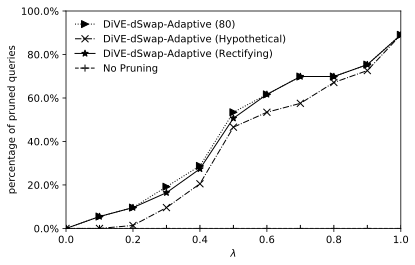
\includegraphics[width=3.0in]{figures/pruning_performance_dswap_rectifying}
		\caption{Rectifying flows}
		\label{fig:Rectifying_flow_column}
	\end{center}
\end{figure}

In order to overcome this issue, rectifying bound of adaptive pruning is proposed. The algorithm of rectifying bound strategy is quite simple as shown in Figure \ref{fig:Rectifying_flow_column}. For instance, there are $V_n$ of number of views in $X$ and user uses PI80. First, the theoritical maximum bound ($ \sqrt{2} $) is used such as in the static approach. In this step, some low-quality views may be pruned. Afterward, As shown in Figure \ref{fig:Rectifying_flow_column}, nine query views are executed in advanced then the estimated maximum bound is obtained from nine executed views and the views in the initialization set $S$. The blue dash line shows the first time of maximum bound is changed from the theoritical bound to the estimated maximum bound (i.e., maximum importance score of views have seen so far). In this step, many low-quality views are pruned. The current version of adaptive pruning scheme will consider these pruned views as the final pruned views, however, rectifying bound mechanism will bring back these pruned views while higher importance score is found in the next iteration. 

\begin{figure}[t]
	\centering
	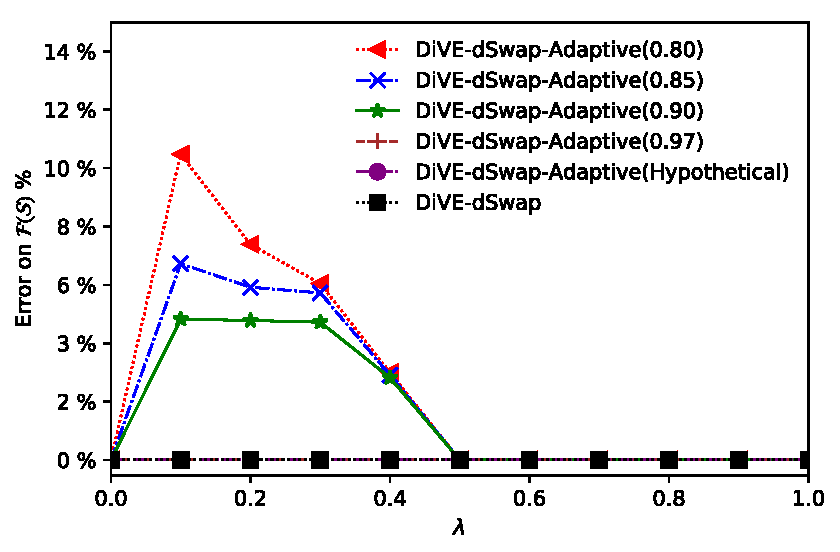
\includegraphics[width=3.6in]{figures/rectifiying_error_f_s_dswap}
	\vspace{-5pt}
	\caption{Impact of Adaptive pruning on $F(S)$}
	\label{fig:pruning_performance_swapd}
\end{figure}



As shown in the example, the higher importance score are found (i.e., $V_{30}$,$V_{55}$,$V_{100}$). All pruned views from the previous steps will be returned and evaluated again while the schemes find higher importance score in the next execution. Then, the maximum bound will be updated to the highest importance score. The scheme will repeat this step until no importance score that higher than the current maximum bound. 

Figure \ref{fig:rectifying_bound} shows the performance of adaptive pruning scheme with rectifying bound strategy compared to without rectifying bound strategy. The pruning peformance after applying rectifying bound strategy quite close to without rectifying bound strategy. Meanwhile, as shown in Figure \ref{fig:rectify_error_fs} there is no effectiveness loss after rectifying bound is implemented. 

\begin{figure}[t]
	\centering
	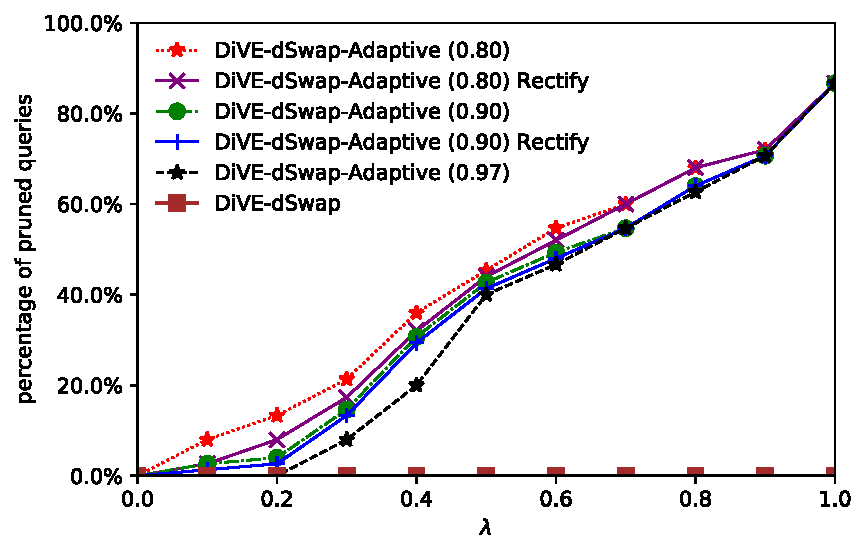
\includegraphics[width=3.6in]{figures/pruning_performance_dswap_adaptive_rectifying_compare}
	\vspace{-5pt}
	\caption{DiVE-dSwap-Adaptive with and without rectifying}
	\label{fig:rectifying_bound}
\end{figure}




\begin{figure}[t]
	\centering
	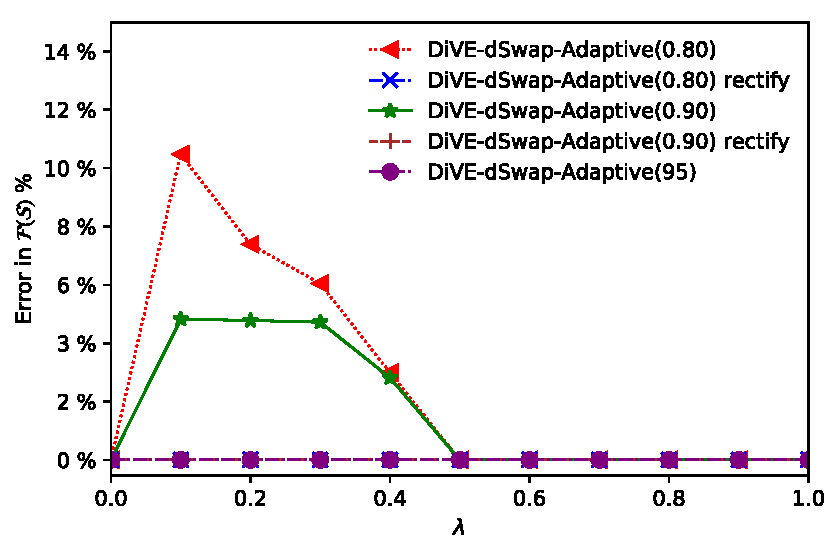
\includegraphics[width=3.6in]{figures/error_fs_rectifying_dswap}
	\vspace{-5pt}
	\caption{Impact of Adaptive pruning on $F(S)$ with and without rectifying}
	\label{fig:rectify_error_fs}
\end{figure}


%However, Figure \ref{fig:rectifying_cost} shows the additional cost of the rectifying bound strategy. 

%The current version of adaptive schemes do not have rectifying bound mechanism.


%
%\begin{figure}
%	\begin{center}
%		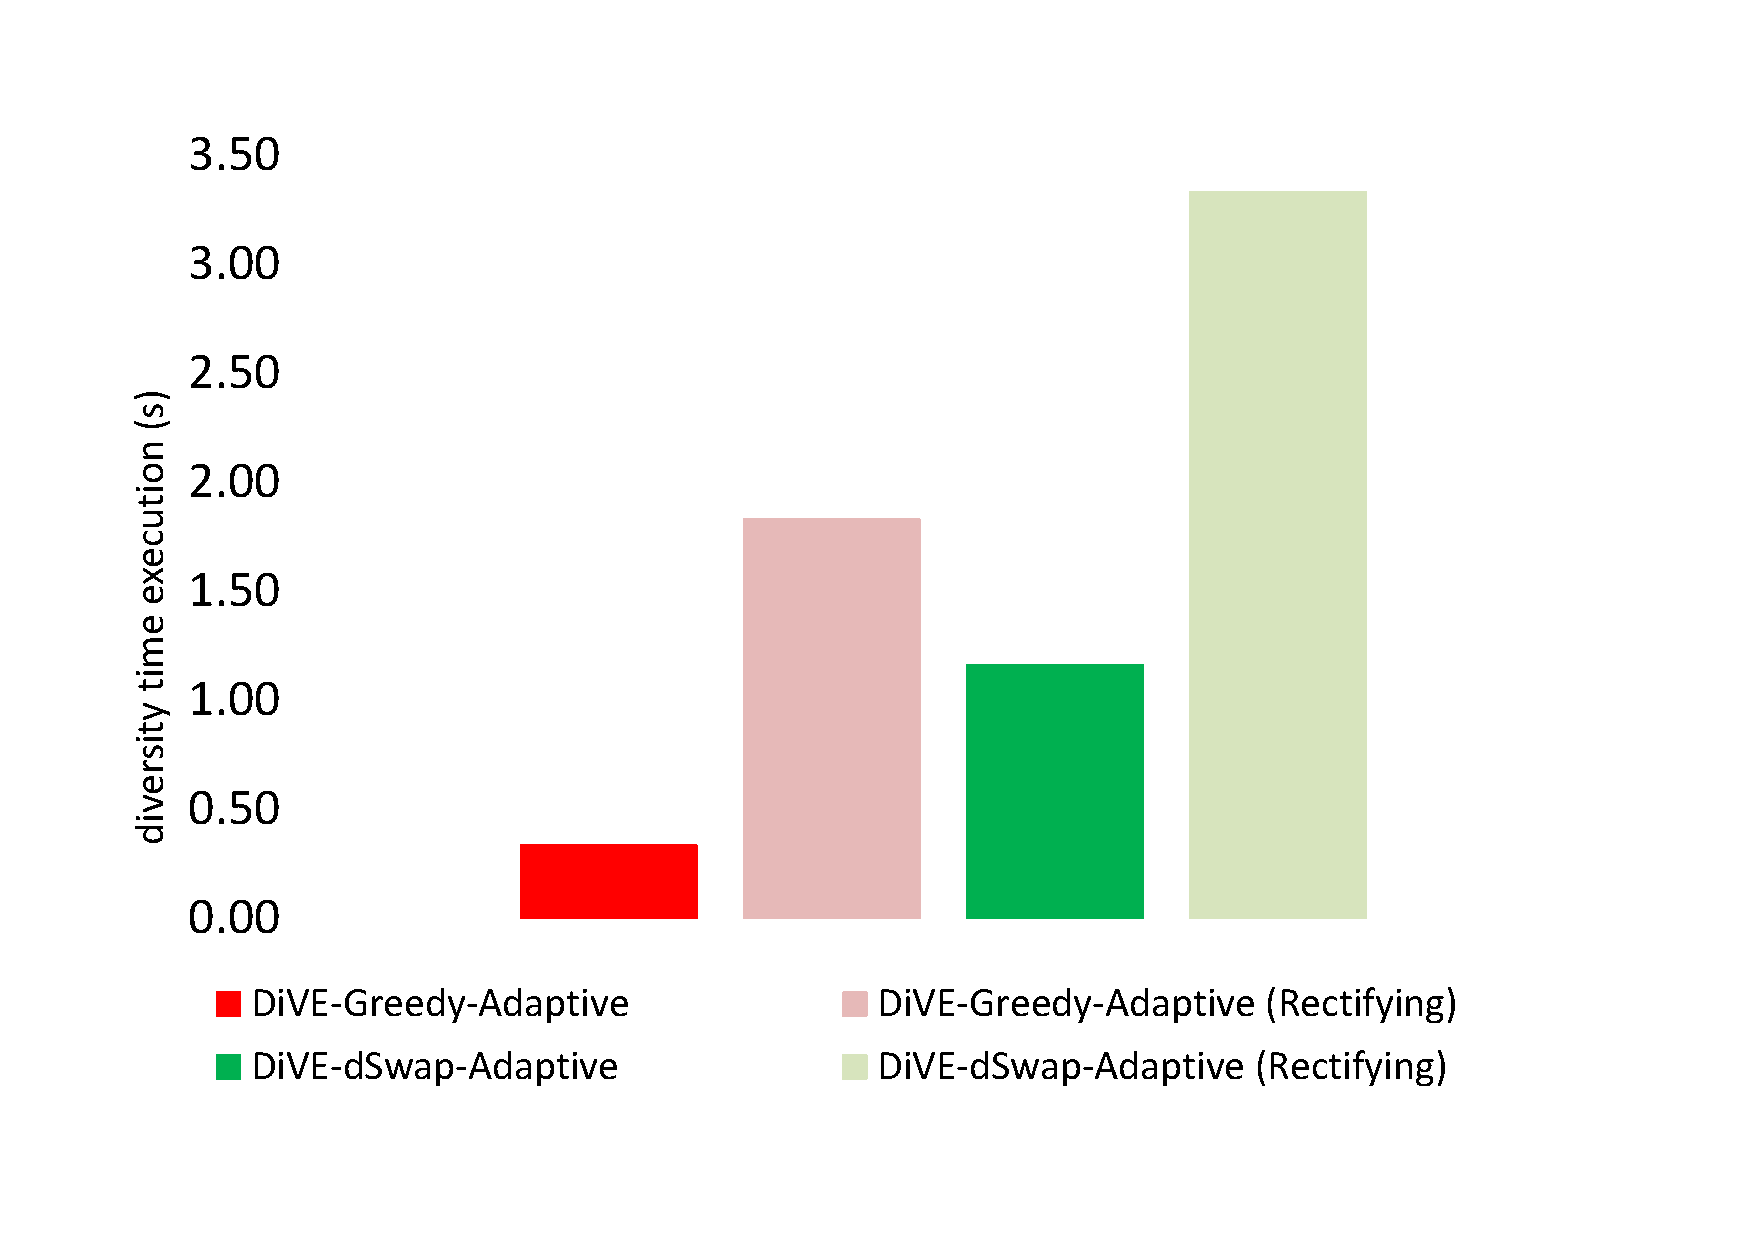
\includegraphics[width=4.0in]{figures/rectifying_cost}
%		\vspace{-8pt}
%		\caption{Rectifying bound strategy cost, $k = 5, \lambda = 0.5$}
%		\label{fig:rectifying_cost}
%		
%	\end{center}
%\end{figure}



%\begin{figure}
%	\begin{center}
%		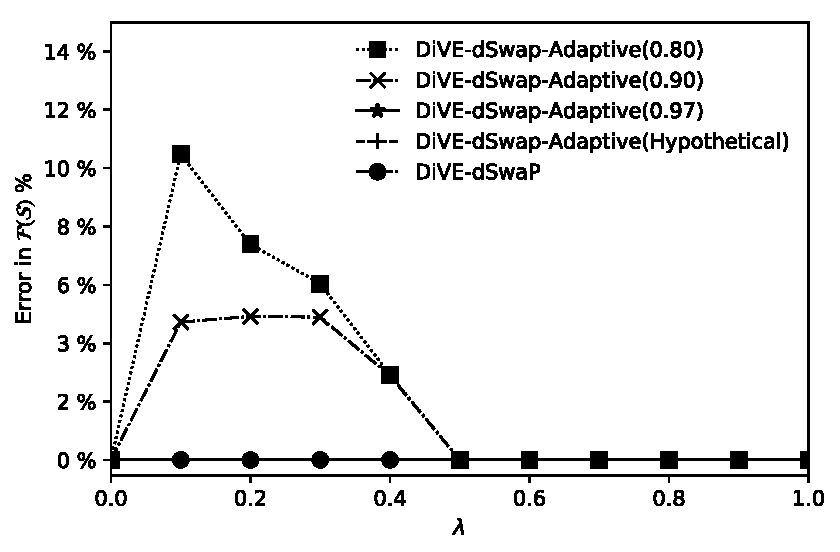
\includegraphics[width=4.0in]{figures/error_f_s}
%		\vspace{-12pt}
%		\caption{Impact of $k$ to diversity computation running on Flights dataset}
%		\label{fig:error_fs_adaptive}
%		
%	\end{center}
%\end{figure}

\section{Query sharing computation}

Beside using pruning, SeeDB used query sharing optimizaation to reduce the query executions. To do query sharing optimization, SeeDB used techniques such as: combine multiple aggregates, combine multiple GROUP BY, and combine target and reference view query. However, pruning and query sharing seem two kinds of orthogonal optimizations. Hence, SeeDB proposed \textit{phased execution framework} which was by dividing dataset to phases. For instance, if we have 100,000 records in our dataset and we use 10 phases, the $i = 4^{th}$ processes records 30,001 - 40,000. 

In fact, SeeDB used partial result of each aggregate view on the fractions and used it to estimate the quality of each view and prune low-quality views in each phase. The query sharing optimization is used to minimize scans on the fraction of dataset in each phase whereas the pruning-based optimization is processed in the end of each phase.

If we see the SeeDB proposed approach, they divided the data to many phases and in the begining of phase, the query sharing computation is applied in the fraction and use that partial result to estimate the quality of view which still under consideration and in the end, the pruning-based optimizataion is applied. Due to of this, I do not think that this query sharing approach is applicable to our work. 

In case of our work, we sorted the remaining views based on $setDist$ score and execute the query view one by one start from the top and we need to know the importance score of executed view in order to get the current $ F(S) $ and to update the maximum bound. We also assume that by sorting the views based on $setDist$ the chance view is similar to others view in the above and below position are low. It means that to do query sharing execution by combining multiple aggregate or GROUP BY is difficult. There is no possibility to collect all views with same aggregate function or GROUP BY then execute in the same time due to we need to know the importance score of each view one by one.     


\end{document}



% Pruning Pseudocode

\begin{algorithm}
	\SetAlgoVlined
	%This is to hide Begin keyword
	\SetKwBlock{Begin}{}{end}
	\KwIn{Set of views V and result set $S$ize k }
	\KwOut{Result set $ S \geq V $, size S = k}  
	$S \leftarrow $ Result set of only diversity\;
	$X \leftarrow  \left[V \backslash S\right]$\;
	$F_{current} \leftarrow 0 $\;
	$  improve \leftarrow  True $\;
	$ max_b  \leftarrow\sqrt{2} $\;
	%$ S_{rectify}  \leftarrow [] $\;
	%$ X_{rectify}  \leftarrow [] $\;
	\While{improve = True}{
		%$ X' \leftarrow [] $\;
		\For{$X_i$ in set $X$}{
			\For{$S_j$ in set $S$}{
				$ d  \leftarrow setDist\left(X_i,S \backslash S_j\right) $\;
				$ 	newX \leftarrow [S_j, X_i, d]$\;
				$ 	X'.append(newX)$\;
			}
		}
		$ 	X' \leftarrow sorted\_by\_d(X') $\;
		$ S' \leftarrow S $\;
		$ rectify  = False $\;
		\eIf{ $ max_b == \sqrt{2} $}{
			\For{$i$ in set $X'$}{
				
				\If{ $ F\left(S'\right) < F\left(S \backslash X'[i][0] \cup X'[i][1], max_b\right) $}{
					$ 	X''.append(X'[i][1])$\;
				}
			}
			
			$n \leftarrow pi - len(S)$\;
			$samples \leftarrow X''[0\colon n]$\;
			$maxI\_S \leftarrow get\_maxI(S)$\;
			$maxI\_samples \leftarrow get\_maxI(samples)$\;
			
			\If{ $ maxI\_S > maxI $}{
				$ maxI \leftarrow maxI\_S$
			}
			\If{ $ maxI\_samples> maxI $}{
				$ maxI \leftarrow maxI\_samples$
			}
			$max\_b \leftarrow maxI$	
			
			\For{$i$ in set $X''$}{
				\For{$j$ in set $S$}{
					\If{ $ F\left(S'\right) < F\left(S \backslash S_j \cup X''[i], max_b\right)  $}{
						$ 	X'''.append(X''[i])$\;
						
					}
					$ I \leftarrow get\_I\_score(X'''[i]) $\;
					\If{ $ F\left(S'\right) < F\left(S \backslash S_j \cup X'''[i], I\right) $}{
						$ S'  \leftarrow S \backslash j \cup X'''[i] $  \;
					}
					\If{ $ I > max_b $}{
						$ max_b \leftarrow I $\;
						$ rectify = True $\;
						$ break (Out\ of\ Loop) $\;
					}
				}
			}
			
		}{ 
			
			
		}
		%
		%\If{ $ F\left(S'\right) > F\left(S\right) $}{
		%	$ S  \leftarrow S'$
		%	$  improve \leftarrow  True $\;
		%	
		%	}{
		%		$improve \leftarrow  False $\;
		%	
		%	}
	}
	%return S
	\caption{\textit{DiVE} dSwap Pruning Rectifying}\label{DiVE-dSwap-Pruning-Rectifying}
\end{algorithm}

\begin{algorithm}
	\LinesNumbered
	\setcounter{AlgoLine}{37}
	% This is to restore vline mode if you did not take the package as \usepackage[linesnumbered,ruled,vlined]{algorithm2e}
	\SetAlgoVlined
	%This is to hide Begin keyword
	\SetKwBlock{Begin}{}{end}
	\Begin{
		\eIf{...}{...}
		{
			
			\For{$X_i$ in set $X'$}{
				\If{ $ F\left(S'\right) < F\left(S \backslash X'[i][0] \cup X'[i][1], max_b\right) $}{
					$ 	X''.append(X'[i][1])$\;
				}
				$ I \leftarrow get\_I\_(X''[i]) $\;
				\If{ $ F\left(S'\right) < F\left(S \backslash S_j \cup X''[i], I\right) $}{
					$ S'  \leftarrow S \backslash j \cup X''[i] $  \;
				}
				\If{ $ I > max\_b $}{
					$ max\_b \leftarrow I $ \;
					$ rectify = True $\;
					$ break (Out\ of\ Loop) $\;
				}
				
			}
			
		}
		
		\eIf{rectify == True}{
			$improve \leftarrow  True$ \;
			
			
		}{
			
			
			\If{ $ F\left(S'\right) > F\left(S\right) $}{
				$ S  \leftarrow S'$\;
				
			}
			
			\eIf{ $ F\left(S\right) > F_{current} $}{
				$ F_{current}  \leftarrow F\left(S\right) $\;
				$  improve \leftarrow  True $\;
				
			}{
				$improve \leftarrow  False $\;
				
			}
			
		}
		
	}   
	$return S$ 
\end{algorithm}

%\section{Proposed algorithm's Figure}
%We proposed DiVE scheme using two kinds of popular heuristic approach which are Greedy and Swap techniques. Figure \ref{fig:algorithm-figure} shows our proposed scheme technique. In case of Greedy, the set $ S $ is initialized by two most distant views. In each iteration, the best view in $ X $ that can maximize objective function $F(S)$ will be added to the set $ S $. Meanwhile, for the Swap case, the set $ S $ is initialized by the most diverse $  k $ views and in each iteration, all candidates views in $ X $ will be interchanged to set $ S $ and view which can improve the current objective function $F(S)$ will replace a view in set $ S $.
%
%The $setDist$ score is used to sort all candidate views in $ X $, the highest score means that views is more diverse to set $ S $. The current bound is utilized to compute the estimate utility of each candidate view. First, the theoritical maximum bound ($ \sqrt{2} $) is used and this bound is updated while the actual importace score of view has been known. To avoid the wrong current bound, samping based on prediction interval is used. Before running the program, user needs to defined what PI that she wants to use. For instance, while users set PI to 80 then after 9 views is executed the current bound will be updated to the maximum bound which have seen so far. The most used PI can be defined as following: 
%
%\begin{itemize}[noitemsep]
%	\item PI80: need to execute 9 views
%	\item PI85: need to execute 12 views
%	\item PI90: need to executes 20 views
%	\item PI95: need to executes 40 views
%	\item PI97: need to executes 60 views
%\end{itemize}
%
%
%\begin{figure}
%	\begin{center}
%		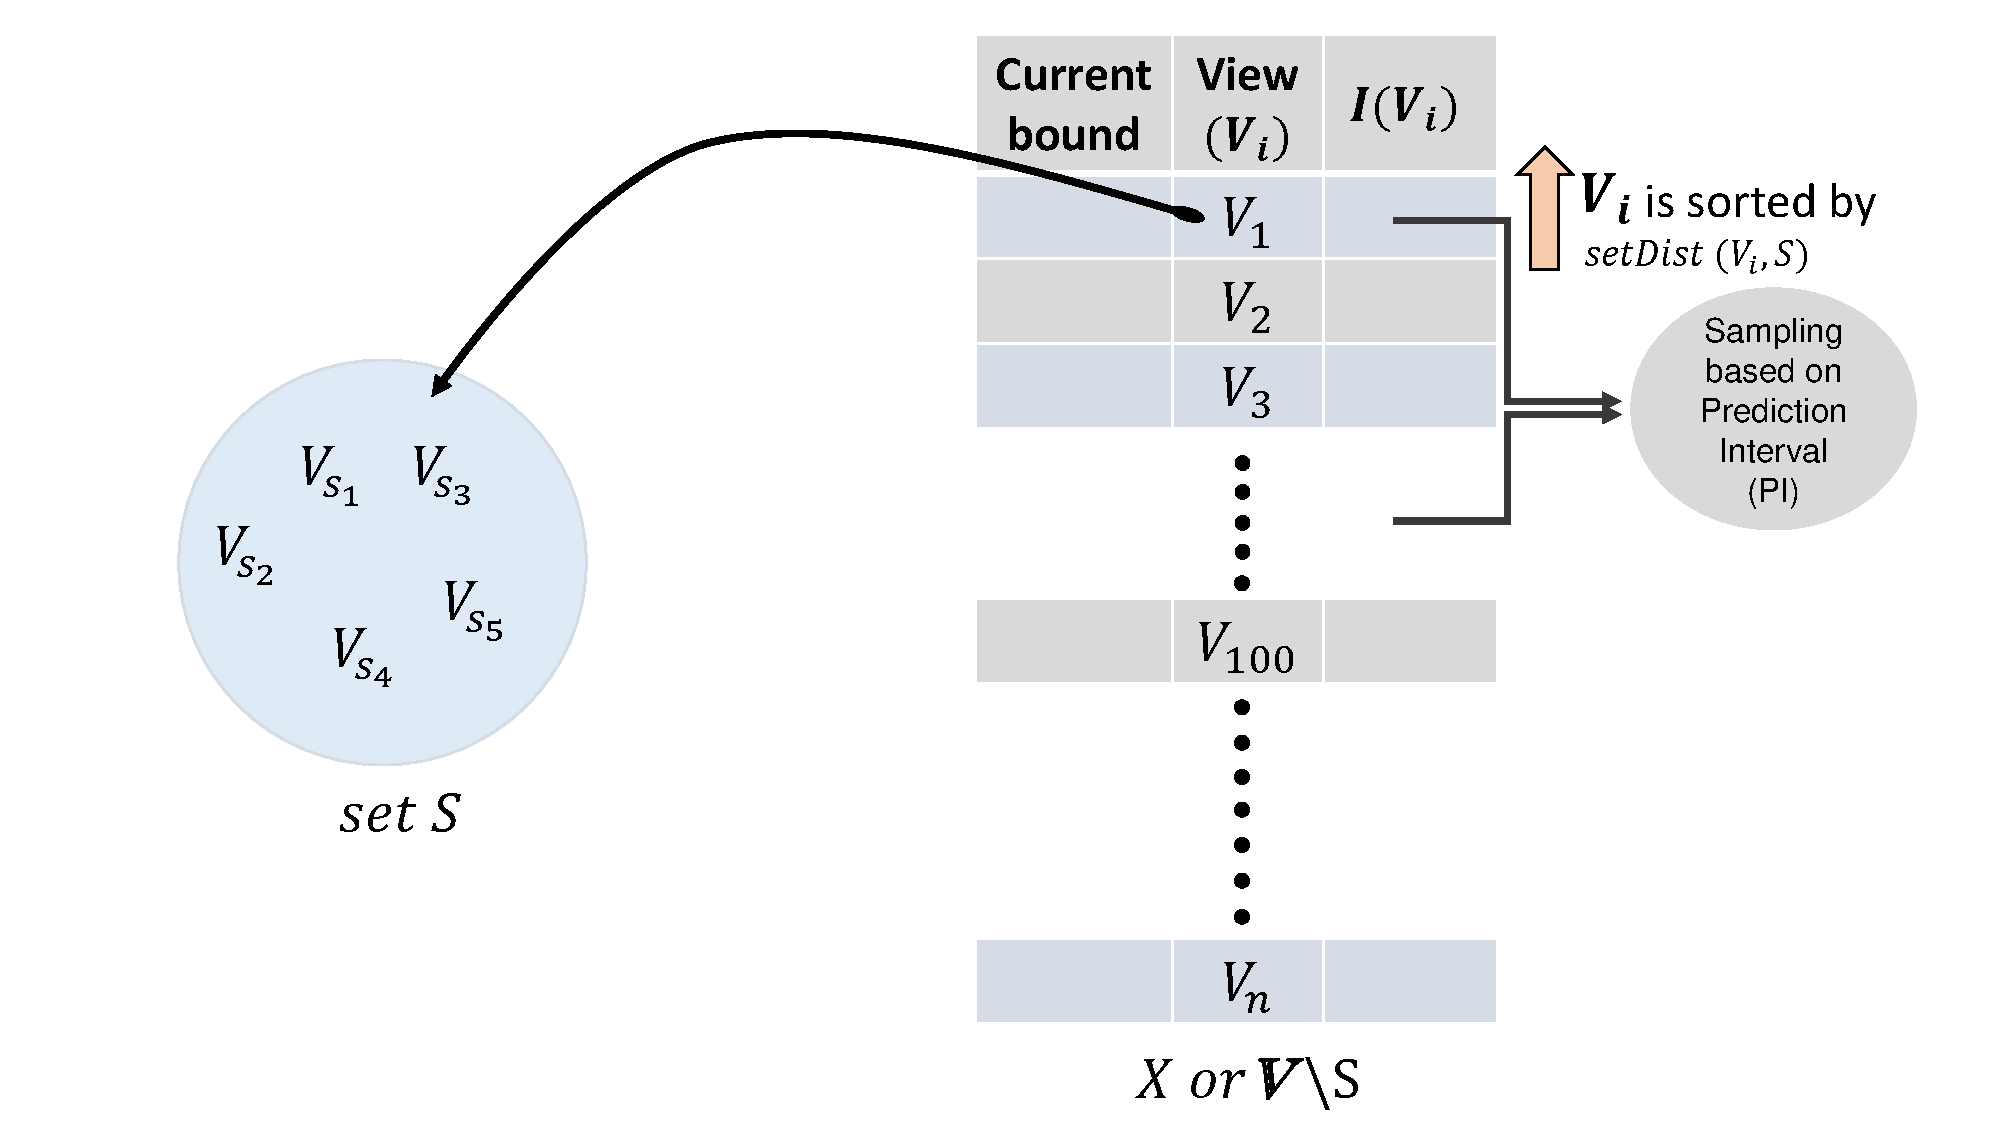
\includegraphics[width=5.0in]{figures/Algorithm}
%		\vspace{-12pt}
%		\caption{Utilizing $setDist$ score to sort candidate views and update current maximum bound to optimize the pruning performance}
%		\label{fig:algorithm-figure}
%		
%	\end{center}
%\end{figure}


%For the general case, Euclidean distance $d$ is defined as following: 
%$d = \sum{(x-y)^2} = \sum x^2 + \sum y^2 - 2\sum xy$. Given that in probability vectors all values are nonnegative, $d$ is max when the last term is zero, then $d = \sum x^2 + \sum y^2$.
%
%All values are between 0 and 1 (sum up to 1), $\sum x = \sum y = 1$. In such a vector, its theoretical maximum is attained when all its entries are 0 except one which is 1, it is when $\sum x^2 = \sum x$ and $\sum y^2 = \sum y$. It also follows from the above description, that then $\sum xy$ can very easily happen to be zero (since in each vector there is just single nonzero element).
%\newline

%Example maximum condition for two bins case: 
%\newline
%
%$\sum a = \sum b = 1$, $a , b \geq 0$
%\newline
%
%$(\sum a)^2 + (\sum b)^2 \geq \sum a^2 + \sum b^2$
%\newline
%
%$(\sum a)^2 + (\sum b)^2 \geq \sum a^2 + \sum b^2 - \sum 2ab $ 
%\newline
%
%$(\sum a)^2 + (\sum b)^2 \geq \sum (a^2 +  b^2 -  2ab)  $ 
%\newline
%
%$(\sum a)^2 + (\sum b)^2 \geq \sum (a-b)^2  $ 
%\newline
%
%$1 + 1 \geq \sum (a-b)^2  $ 
%\newline
%
%$\sqrt{2} \geq \sqrt{\sum (a-b)^2}  $ 
%\newline

%Max-sum is bi-criteria objective function to maximize the sum of the relevance and dissimilarity of the selected set, which can be defined as follows:
%
%\begin{equation}
%F\left(S\right) =  \left(1-\lambda\right) * I\left(S\right) + \lambda * f\left(S,D\right)
%\label{objectif_function}
%\end{equation}
%
%Where, 
%$ I\left(S\right)= \sum_{i=1}^{k} \dfrac{I(V_i )}{I_u}, V_i  \in S $ and $ f\left(S,D\right)= \dfrac{1}{k\left(k-1\right)}  \sum_{i=1}^{k} \sum_{j>i}^{k} D\left(V_i,V_j\right) ,V_i,V_j  \in S $
%\newline
%
%Meanwhile, Max-min diversification is the bi-criteria objective function that maximize the \textit{minimum} relevance and dissimilarity of the selected set. Based on the work of Gollapudi (An axiometic approach for result diversificaiton), this objective function can be defined as follows: 
%
%\begin{equation}
%F\left(S\right) = (1-\lambda) * \underset{u \in S} {\mathrm{min}} \ w\left(u\right)  + \lambda * \underset{u,v \in S} {\mathrm{min}} d\left(u,v\right)
%\end{equation}
%
%While Max-min diversification is to maximize the minimum of importance score, I am not sure this approach is relevant or not for our work. 